\documentclass[11pt]{article}
\usepackage{amsmath,amssymb,float,amsfonts,enumitem,tcolorbox,hyperref,url}



%!TEX root = EM_singular_models.tex

% PDF margin etc settings
\setlength{\textwidth}{\paperwidth}
\addtolength{\textwidth}{-6cm}
\setlength{\textheight}{\paperheight}
\addtolength{\textheight}{-4cm}
\addtolength{\textheight}{-1.1\headheight}
\addtolength{\textheight}{-\headsep}
\addtolength{\textheight}{-\footskip}
\setlength{\oddsidemargin}{0.5cm}
\setlength{\evensidemargin}{0.5cm}

\long\def\comment#1{}
\definecolor{battleshipgrey}{rgb}{0.52, 0.52, 0.51}
\definecolor{darkgray}{rgb}{0.66, 0.66, 0.66}
\definecolor{darkgreen}{rgb}{0.0, 0.2, 0.13}
\definecolor{darkspringgreen}{rgb}{0.09, 0.45, 0.27}
\definecolor{dukeblue}{rgb}{0.0, 0.0, 0.61}
\definecolor{olivedrab7}{rgb}{0.24, 0.2, 0.12}
\definecolor{darkblue}{rgb}{0.0, 0.0, 0.55}
\definecolor{darkscarlet}{rgb}{0.34, 0.01, 0.1}
\definecolor{candyapplered}{rgb}{1.0, 0.03, 0.0}
\definecolor{ao(english)}{rgb}{0.0, 0.5, 0.0}
\definecolor{applegreen}{rgb}{0.55, 0.71, 0.0}
\definecolor{orange}{rgb}{1.0, 0.65, 0.0}

\newcommand{\red}[1]{\textcolor{red}{#1}}
\newcommand{\blue}[1]{\textcolor{blue}{#1}}
\newcommand{\green}[1]{\textcolor{green}{#1}}
\newcommand{\orange}[1]{\textcolor{orange}{#1}}
\newcommand{\highlight}[1]{\textcolor{applegreen}{#1}}

\newcommand{\rdcomment}[1]{{\bf{{\red{{RD --- #1}}}}}}
\newcommand{\yccomment}[1]{{\bf{{\orange{{YC --- #1}}}}}}

\renewcommand{\vec}[1]{\mathbf{#1}}
\newcommand{\mat}[1]{\mathbf{#1}}

% Basic Math notations
% Dimension etc.
\newcommand{\dims}{\ensuremath{d}}
\newcommand{\real}{\ensuremath{\mathbb{R}}}
\newcommand{\naturalnum}{\ensuremath{\mathbb{N}}}
\newcommand{\Ind}{\ensuremath{\mathbb{I}}}
% Probability
\newcommand{\borel}{\ensuremath{\mathcal{B}}}
\newcommand{\lebesgue}{\ensuremath{\mathfrak{L}}}
\newcommand{\powerset}{\ensuremath{\mathfrak{P}}}
\newcommand{\lebesguemeasure}{\ensuremath{\lambda}}
\newcommand{\ball}{\ensuremath{\mathbb{B}}}
\newcommand{\Exs}{\ensuremath{{\mathbb{E}}}}
\newcommand{\Prob}{\ensuremath{{\mathbb{P}}}}
\newcommand{\Law}{\mathcal{L}}
\newcommand{\Normal}{\ensuremath{\mathcal{N}}}
\newcommand{\Ber}{\ensuremath{\mbox{Ber}}}
\newcommand{\Ent}{\text{Ent}}
\newcommand{\Var}{\text{Var}}


% Brackets
\newcommand{\brackets}[1]{\left[ #1 \right]}
\newcommand{\parenth}[1]{\left( #1 \right)}
\newcommand{\bigparenth}[1]{\big( #1 \big)}
\newcommand{\biggparenth}[1]{\bigg( #1 \bigg)}
\newcommand{\braces}[1]{\left\{ #1 \right \}}
\newcommand{\abss}[1]{\left| #1 \right |}
\newcommand{\angles}[1]{\left\langle #1 \right \rangle}
\newcommand{\ceils}[1]{\left\lceil #1 \right \rceil}
\newcommand{\floors}[1]{\left\lfloor #1 \right \rfloor}
\newcommand{\tp}{^\top}

% Some vector/matrix norms
\newcommand{\matnorm}[3]{|\!|\!| #1 | \! | \!|_{{#2}, {#3}}}
\newcommand{\matsnorm}[2]{\left|\!\left|\!\left| #1 \right|\!\right|\!\right|_{{#2}}}
\newcommand{\vecnorm}[2]{\left\| #1\right\|_{#2}}



\title{STAT 154: Project 2 Clouds Exploration In The Arctic}
\author{Yang Xiang 3034504578\\
Zhihua Zhang  3034504526}
\date{}

\usepackage{Sweave}
\usepackage{multirow}
\begin{document}
\Sconcordance{concordance:PROJ2_write-up.tex:PROJ2_write-up.Rnw:%
1 6 1 1 7 6 1 1 0 15 1 1 17 1 6 7 0 1 2 5 1 1 13 1 2 9 1 1 5 2 4 19 1 1 %
9 1 7 1 1 1 40 1 1 1 8 5 1 1 8 7 1 1 14 3 0 1 1 2 0 1 1 3 0 1 2 4 1 1 %
14 3 0 1 1 2 0 1 1 3 0 1 2 7 1 1 43 1 2 4 1 1 41 1 2 5 1 1 22 1 17 62 1}


\maketitle


\section{Data Collection and Exploration}
\begin{enumerate}[label=(\alph*)]
\item Summary of the paper:\par
\quad As am important part of environmental protection, Earth's climate, takes up more and more attention. From the conclusion of Global climate models, it is very worthwhile to study the climate in the Arctic. Since the accuracy Arctic-wide measurements greatly is essential, the paper aims at proposing two new operational Arctic cloud detection algorithms.\par
\quad To precisely ascertain the cloud pattern, the paper uses the data produced by MISR. Using nine cameras and four spectral bands, MISR collects useful and gigantic data from all 233 paths on a cycle of 16 days and each path is divided into 180 blocks.\par
\quad At last, three physical features $CORR, SD_{An}$ and $NDAI$ indeed contain sufficient information. And the ELCM algorithm is more accurate, has better spatial coverage, and generates probability labels for partly clouds by training QDA.\par
\quad Moreover, the paper not only provides a pratical method to detect cloud in the Arctic, but also set a good example for future statisticians use their power of statistical thinking to influence the world.

\item Summary of data, map plots and pattern observation:\par
\begin{enumerate}


\item[(i)] Summary of data:\par
\quad For Image 1: clear, uncertain and cloudy regions are percents $43.78\%,38.46\%,17.76\%$.\par \quad For Image 2: clear, uncertain and cloudy regions are percents $37.25\%,28.64\%,34.11\%$.\par
\quad For Image 3: clear, uncertain and cloudy regions are percents $29.29\%,52.27\%,18.44\%$.

\item[(ii)] Maps Plots:\par
\quad We did well-labeld map using x, y coordinates baeds to expert labels in figure \ref{Well_label_plot}.
\begin{figure}[h!]
	\centering
	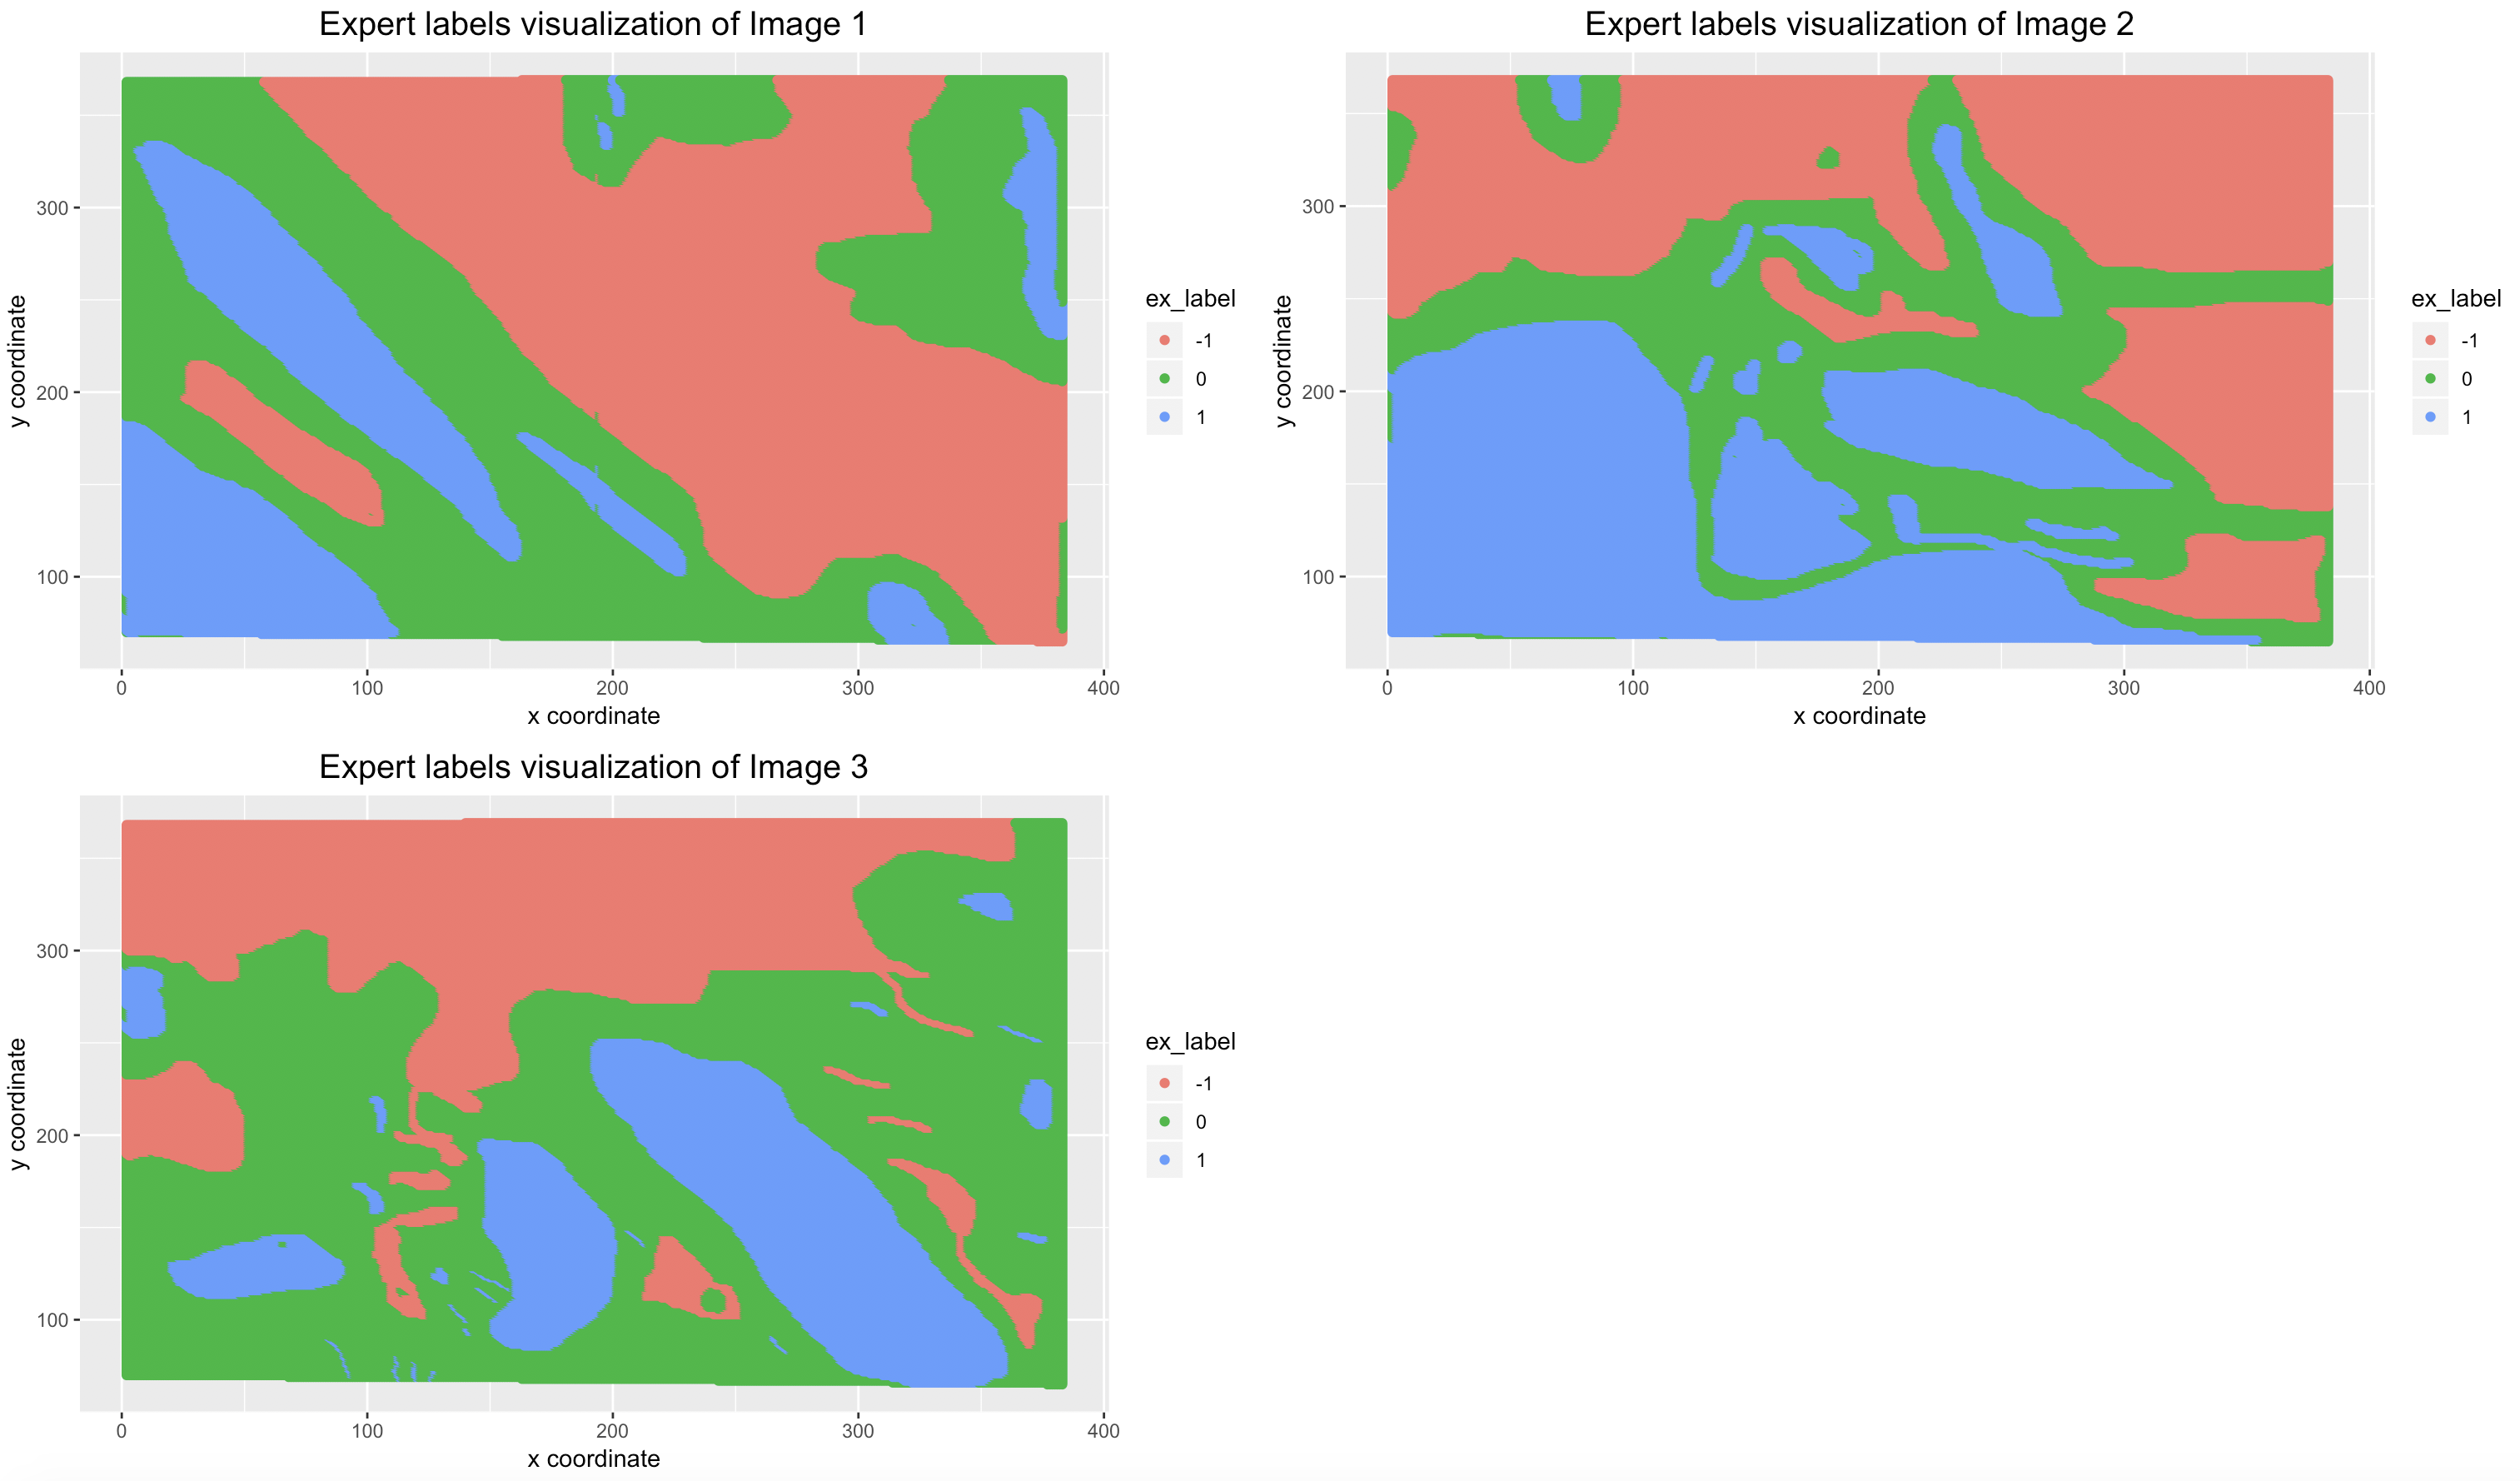
\includegraphics[width = 12cm,height = 7cm]{Figure/map_plot}
	\caption{Well-labeled maps using expert labels}
	\label{Well_label_plot}
\end{figure}

\item[(iii)] Pattern observation:\par
\quad For Image 1: cloud-free regions are mostly in the northeast, cloudy surface locate mainly in the southwest and the uncertain parts, which transits from one to another by intuition, indeed lies between them.\par
\quad For Image 2: cloud-free regions are mostly in the north, while cloudy surface locate mainly in the south. And uncertain parts are also in the middle.\par
\quad For Image 3: Similarly to former two images except cloud-free regions are northwest and locate southeast.\par
\quad Thus, there seems to have intrinsic geographic causes, which implies the $i.i.d$ assumption fails here. Otherwise, we should see a disorderly overlap between cloudy and cloud-free areas. 
\end{enumerate}

\item Visual and quantitative EDA:\par
\quad To clearly explore the relation among different features, we visualize their individual shape and pairwise effects to scrutinize. Moreover, the correlations are computed to give quantitative support and all these are shown in figure \ref{PairwisePlot}.
\begin{enumerate}

\begin{figure}[h!]
	\centering
	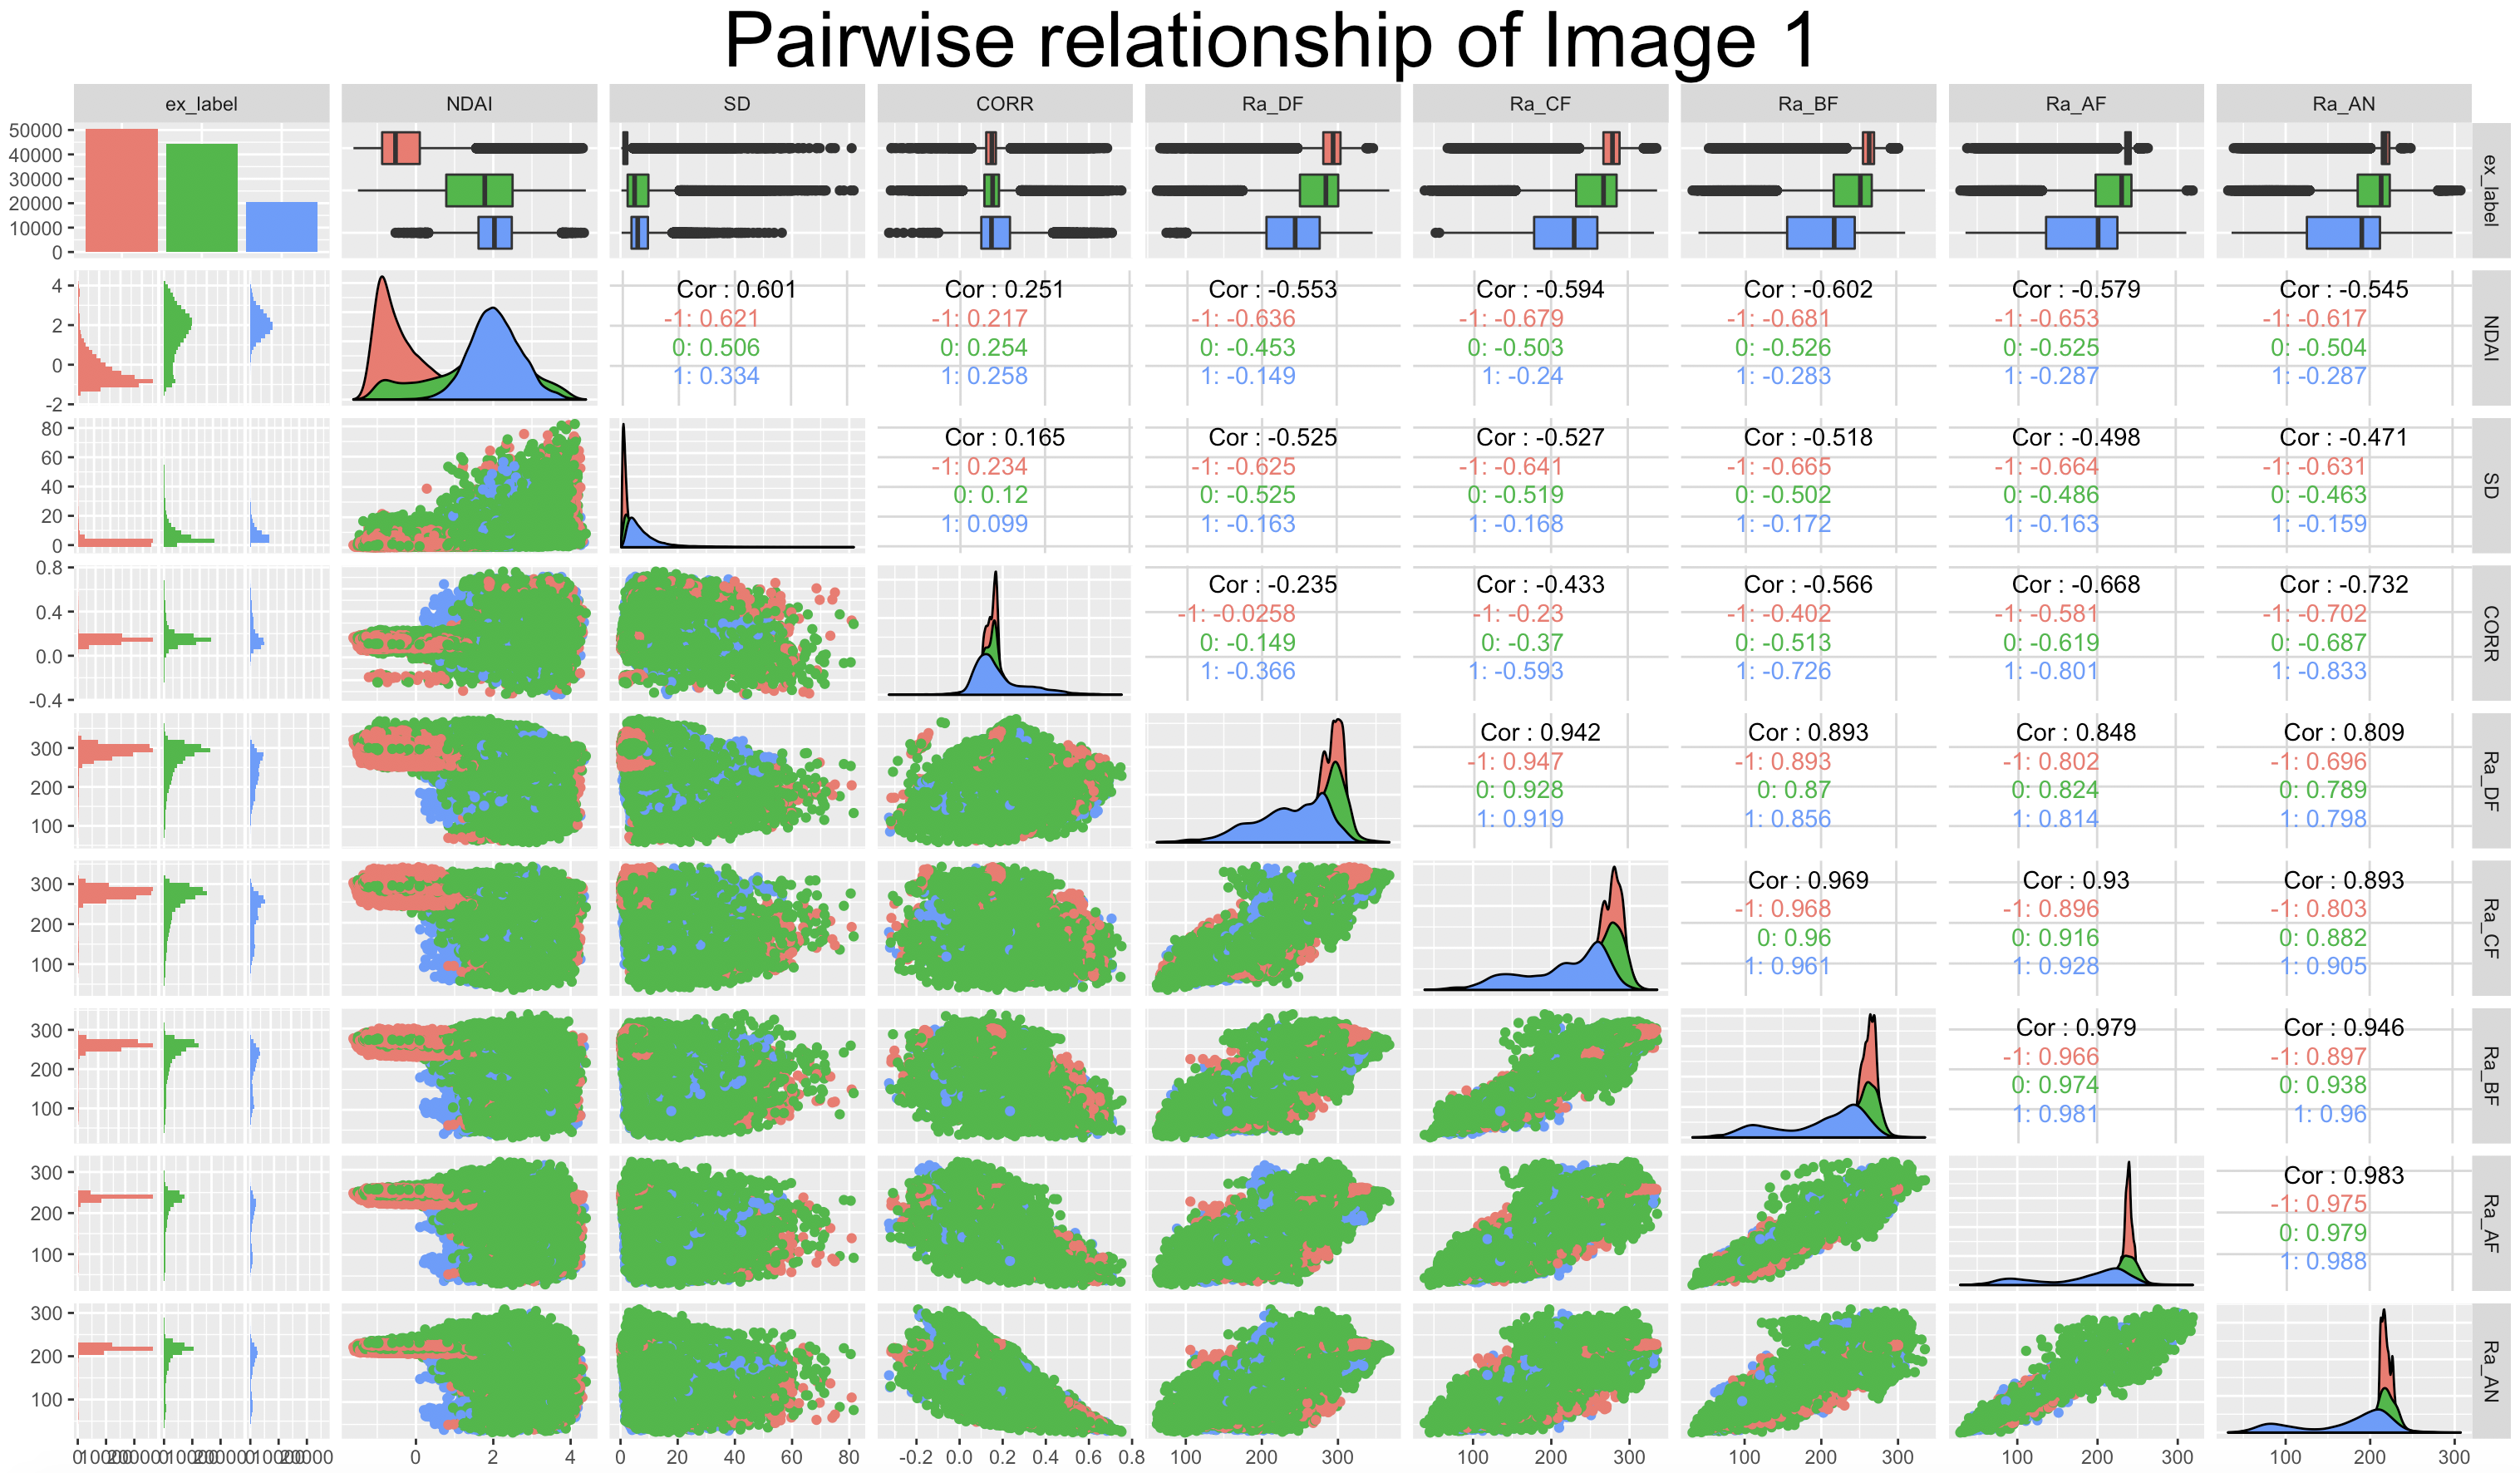
\includegraphics[width = 6cm,height = 6cm]{Figure/Pairwise_1}
	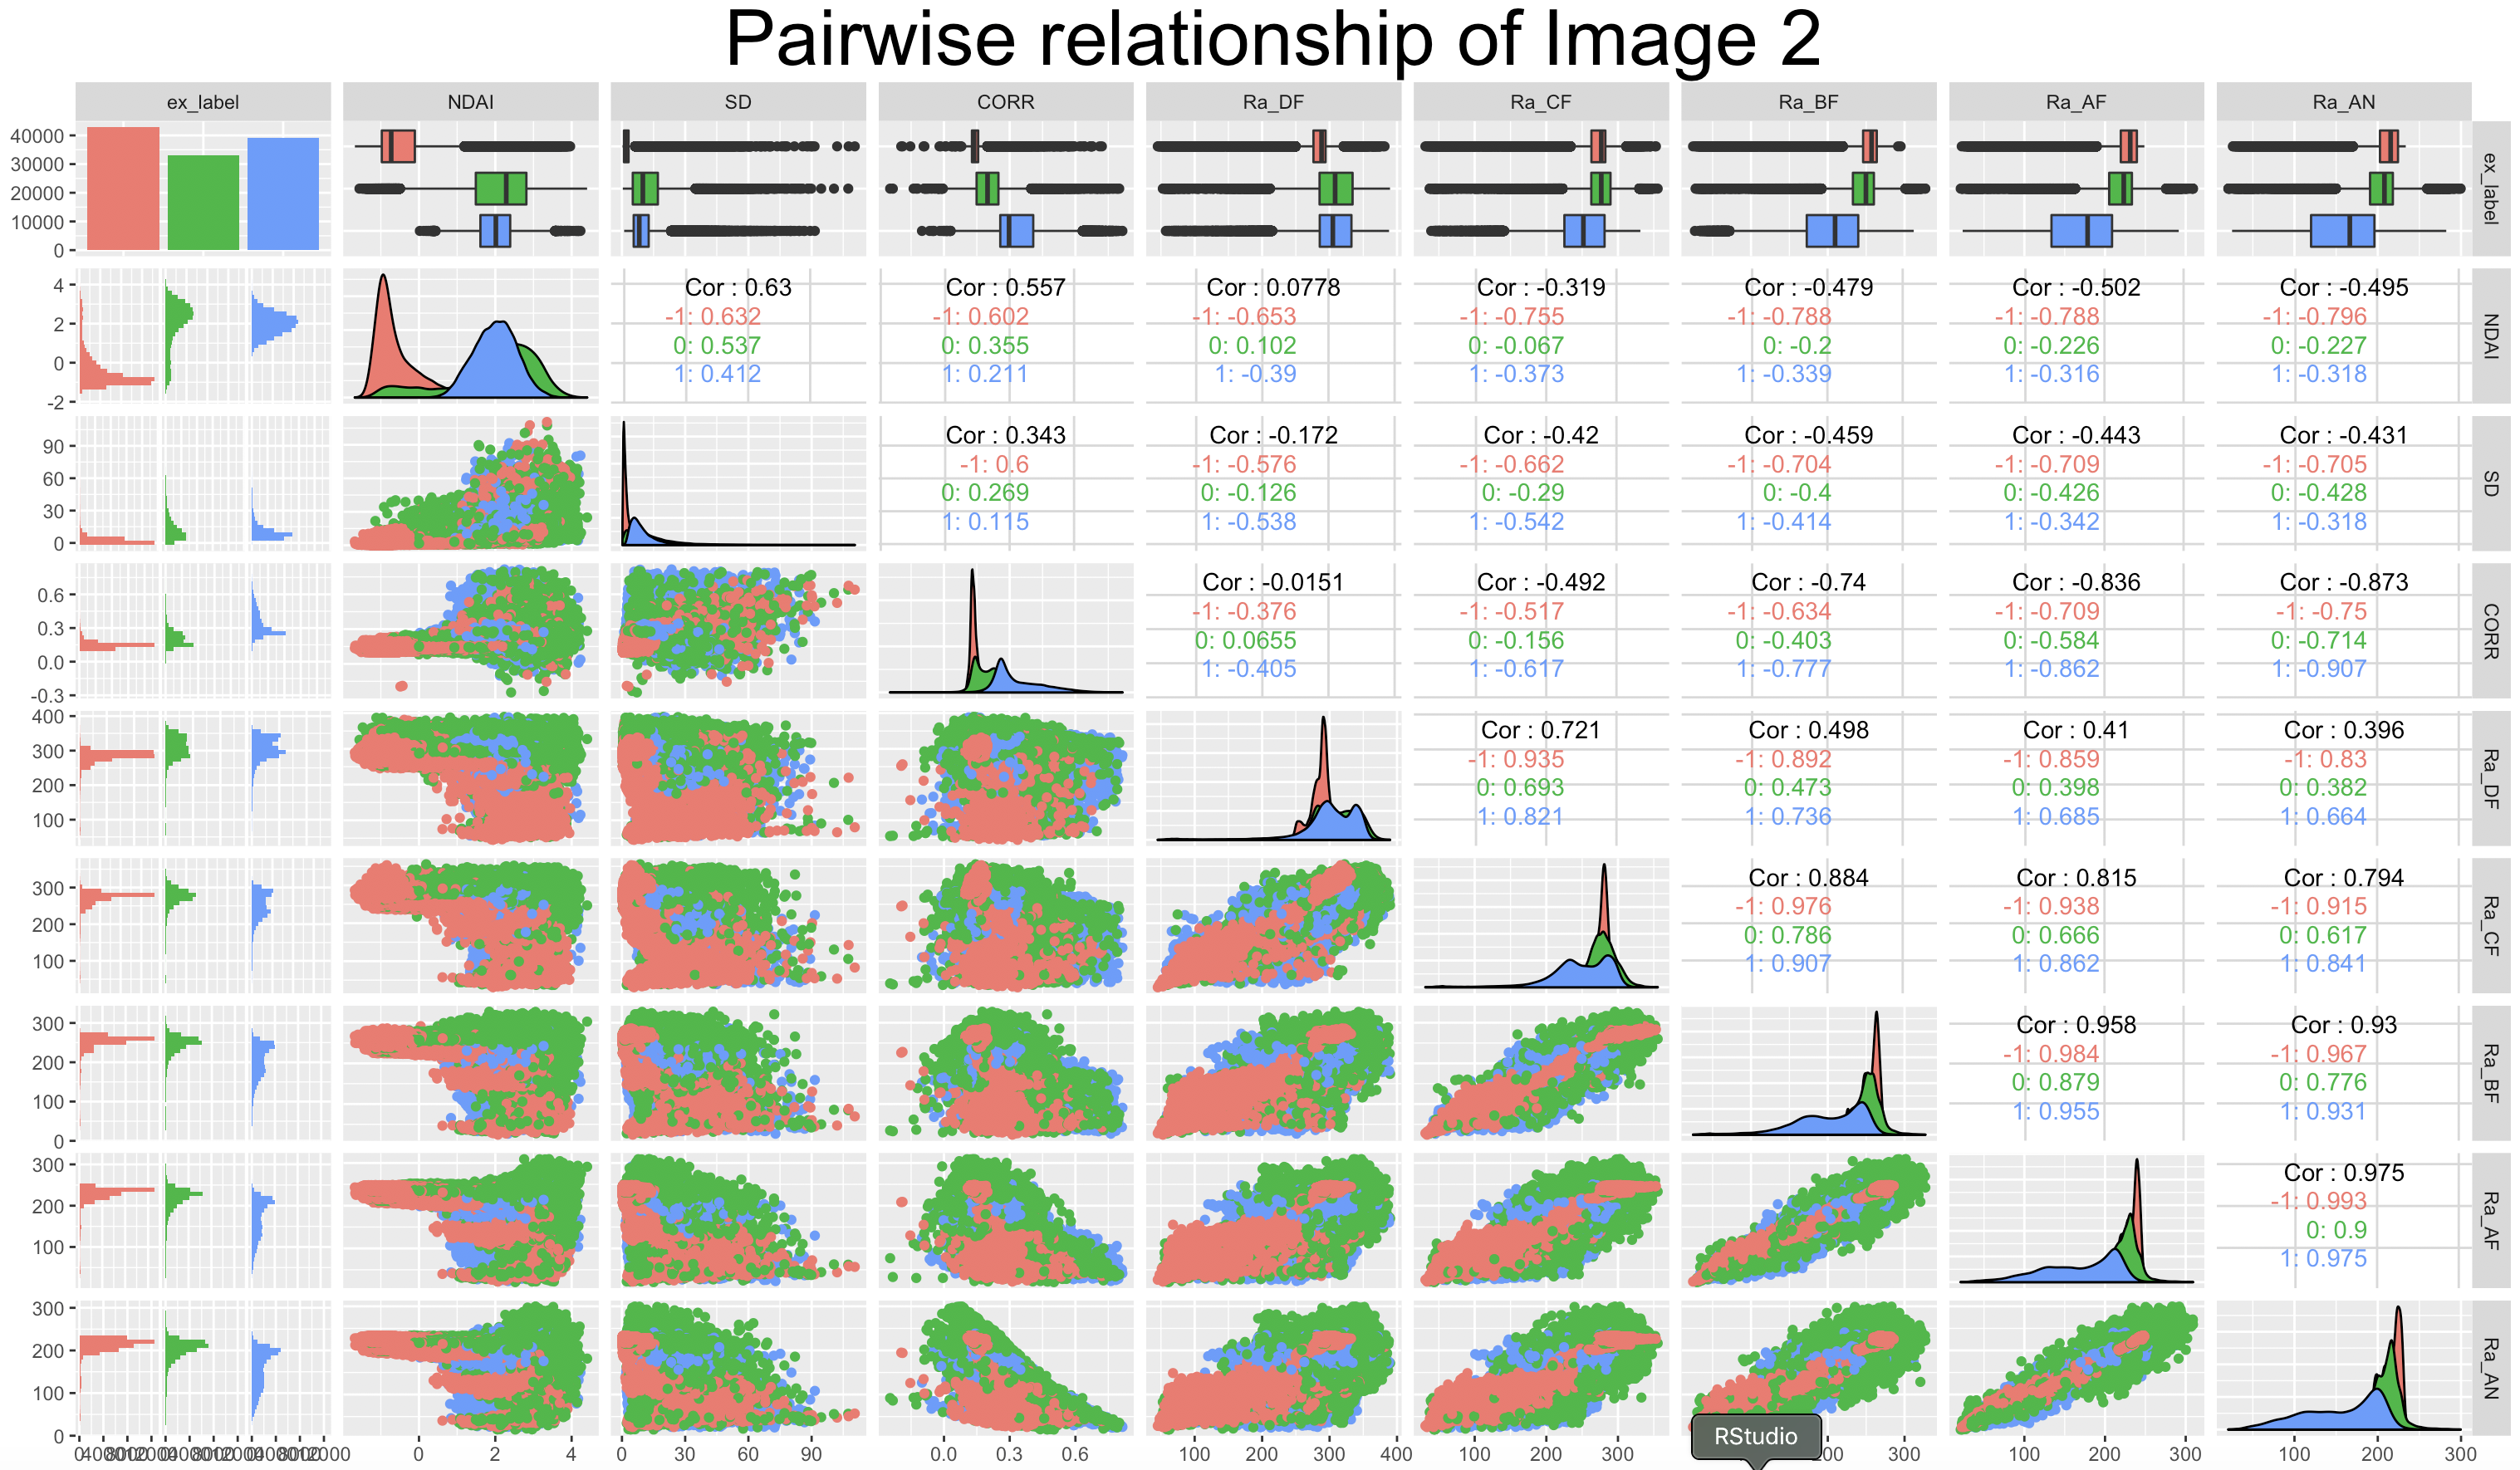
\includegraphics[width = 6cm,height = 6cm]{Figure/Pairwise_2}
	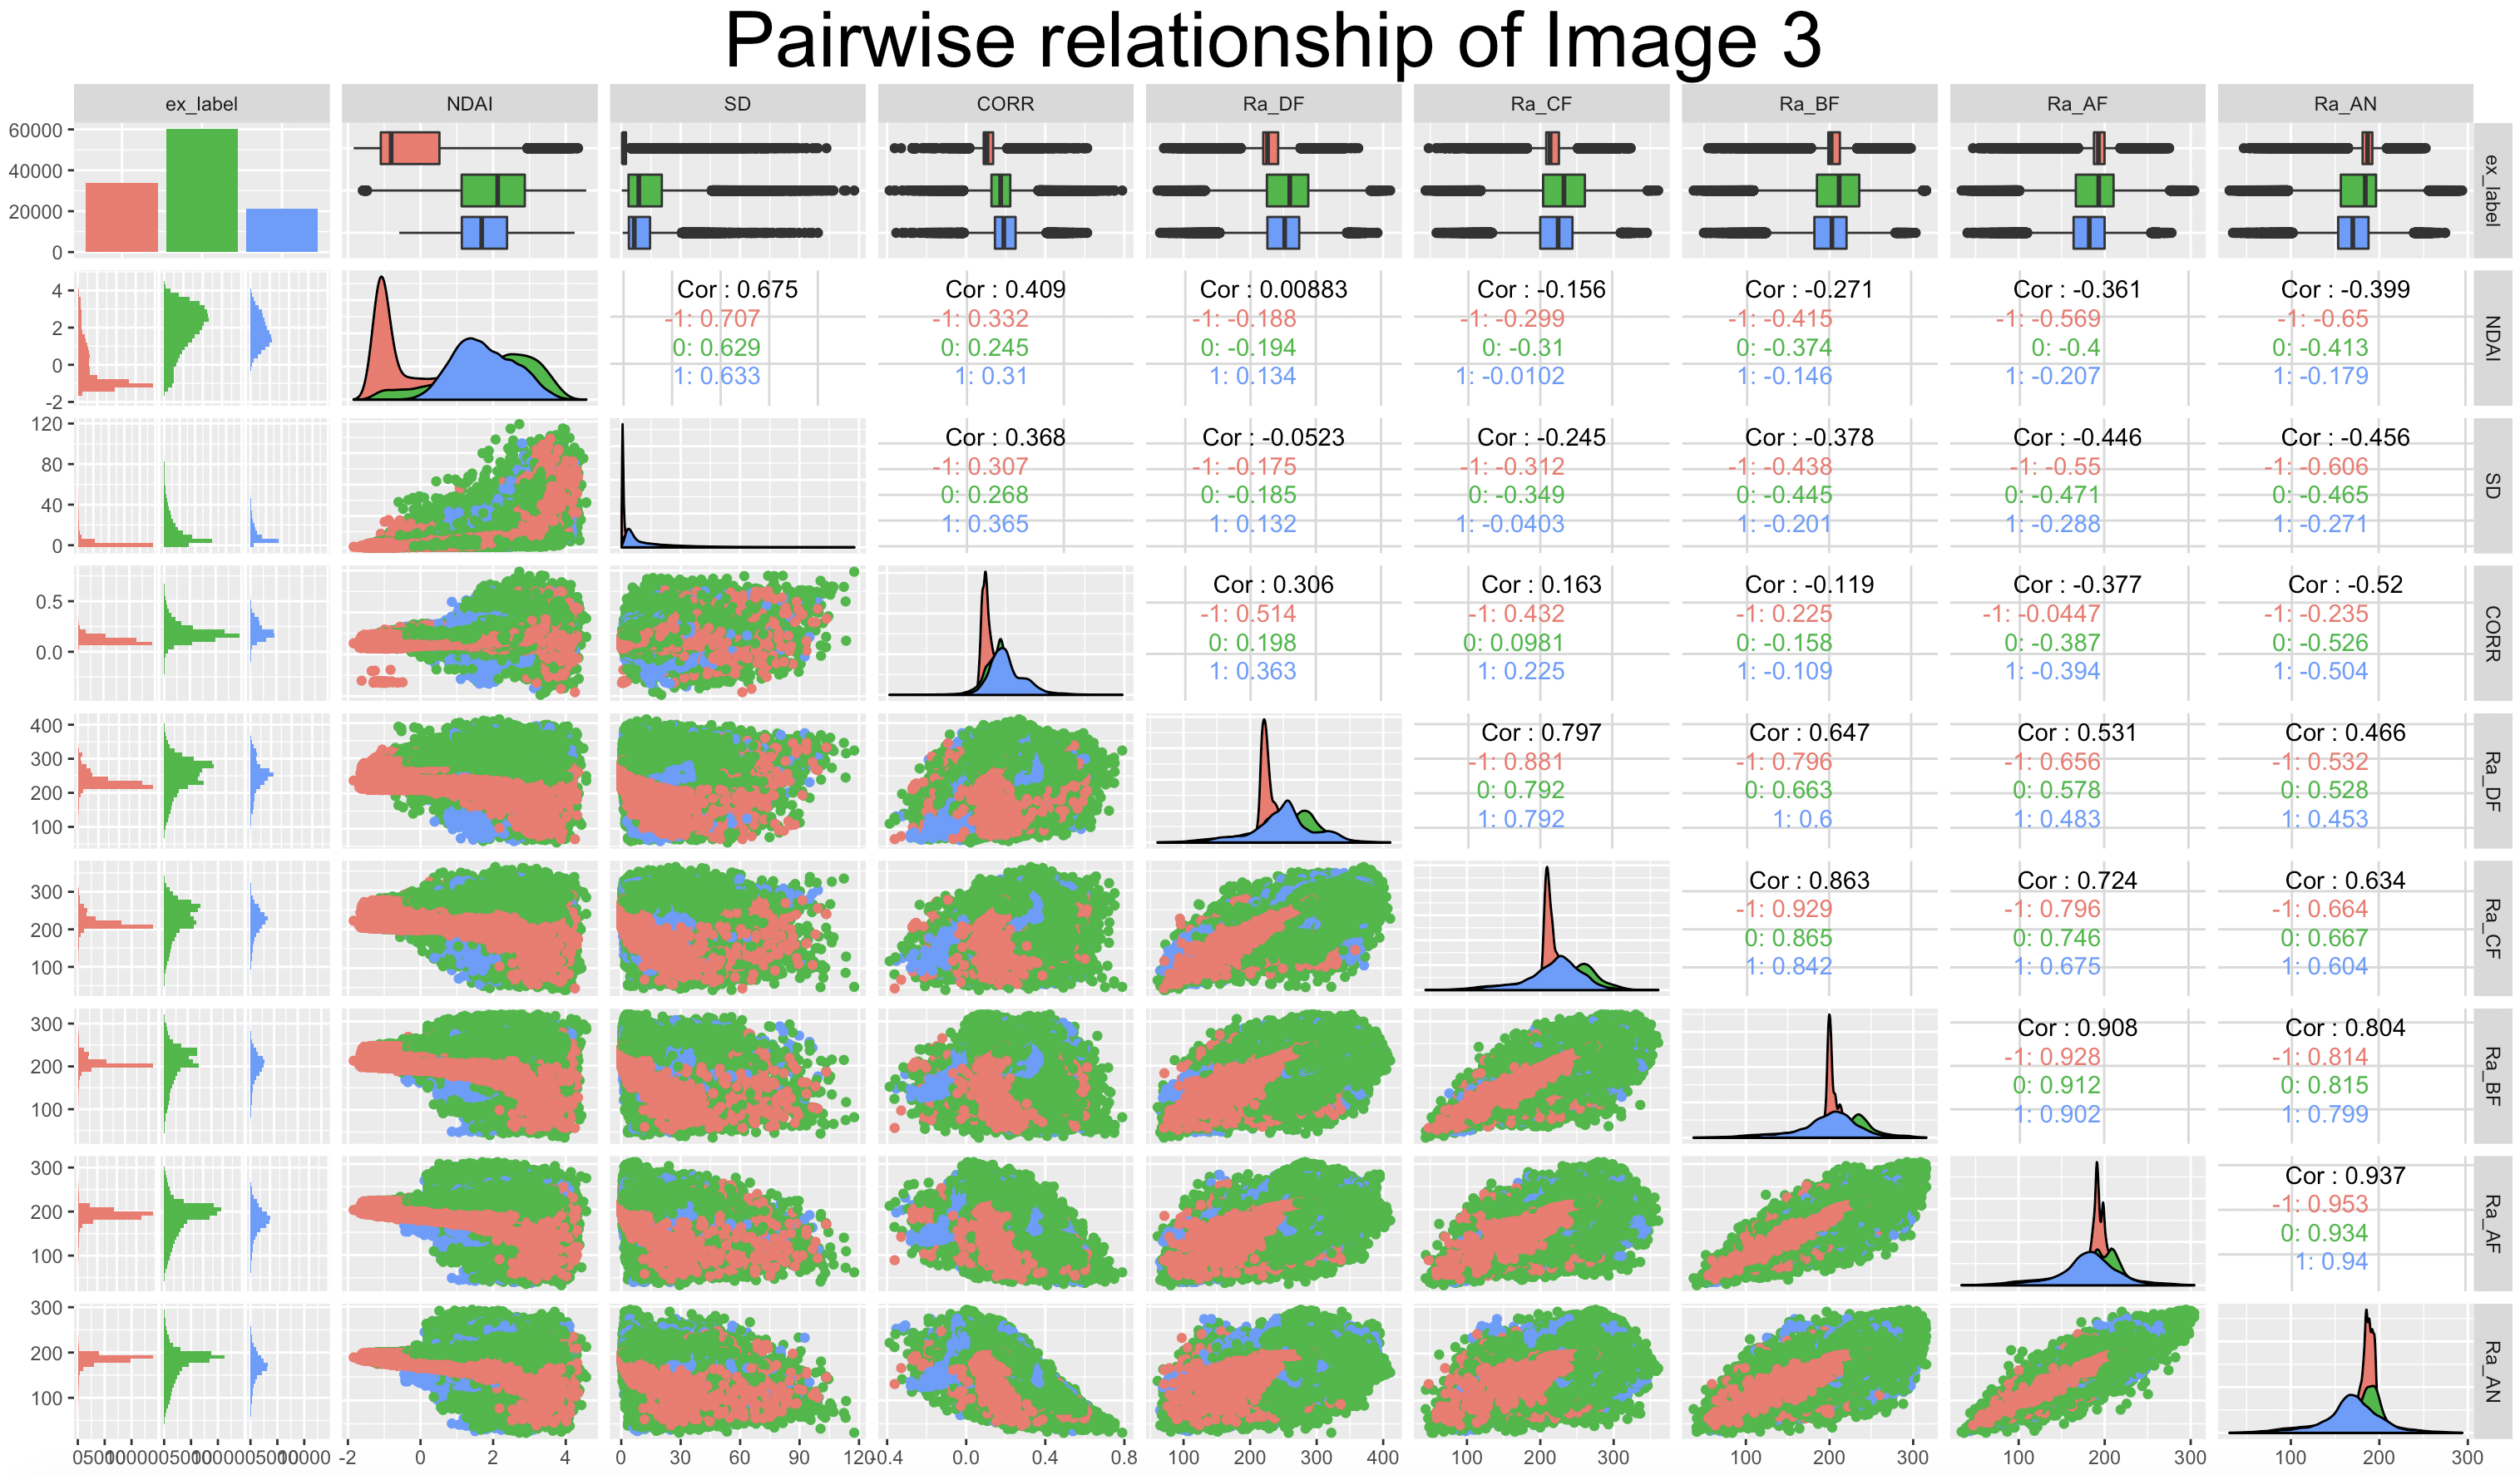
\includegraphics[width = 8cm,height = 6cm]{Figure/Pairwise_3}
	\caption{Pairwise relationship among different features}
	\label{PairwisePlot}
\end{figure}

\item[(i)] Pairwise relationship among features themselves:\par
\quad For themselves: 'SD' and 'CORR' are unimodal, but "NDAI" is bimodal, which is a good signal about separability of clouds.\par
\quad For relationship between each other:(1)There is a significant positive correlation between "NDAI" and "SD"; (2)The five radiance angles are positively correlated to each other; (3)The negative correlation between 'SD', 'CORR' and "NDAI" with radiance gets stronger as the angles gradually come back to nadir direction.

\item[(ii)] Relationship between features the expert labels with the individual features:\par
\quad For "NDAI" and "SD": The separation standard remains same for three images, which is low level indicates clear weather and high value means cloudy areas.\par
\quad For "CORR": The decision rule seems to be unstable, which is similar to "NDAI" and "SD" in Image 2 and Image 3. In Image 1, clear and cloudy regions have highly overlapped "CORR" distribution.\par
\quad For five radiances: "AF" and "AN" have steady decision boundary in three images, but others do not. And the criteria is contrary to the previous one.

\item[(iii)] Differences notification:\par
\quad By EDA about these three images, we observe that on the whole, low levels of "NDAI", "SD" and "CORR" imply the clear areas, whereas high levels of five radiation signify the clear regions. However, it is not immutable, we can observe that there is variation among different images.
\end{enumerate}

\end{enumerate}

\section{Preparation}
Now that we have done EDA with the data, we now prepare to train our model.
\begin{enumerate}[label=(\alph*)]
\item Split the entire data in non-trivial ways:


\begin{enumerate}

\item[(i)] Method 1:

\quad First we decide the proportion of data assigned to three sets: training $60\%$, validation $20\%$, and test $20\%$. The reason is that we truly want to have a lot of test and validation data to ensure robustness, but we still need enough data to train which makes our model grow healthily.\par
\quad Then, considering the existence of spatial dependency, our data is not i.i.d here. We will lose or even get wrong information if we do ramdom spliting imprudently, because we may destroy the dependent structure. In this way, to remain this dependency, we divide our data to block/cluster, then do shuffling and sampling. The gist is that we find if we find weather is cloudy at some position, its neighborhood inclines to be cloudy as well, and so does the clear area. Thus, block-sampling may work well in a way, and for reproductivity, we set random seed as '2019' here.\par
\quad Furthermore, letting blocks have same size is unapt because the number of pixels contained in each block is different. Thus, we determine the block size according to quantiles of coordinate x and y. For example, $block_{ij}$ has length $q_{x,\frac{i}{n}}-q_{x,\frac{i-1}{n}}$ and width $q_{y,\frac{j}{n}}-q_{y,\frac{j-1}{n}}$, where $n^2$ is the total blocks. Here, we choose $n^2=225$.

\item[(ii)] Method 2:

\quad We still follow the rule that spliting data as training, validation and test sets with size 60$\%$, 20$\%$ and 20$\%$ respectively. Moreover, we believe that the block-sampling trick captures the dependency correctly.\par
\quad Thus, we only need to consider the hyperparameter, total number of blocks, which is crucial towards training a good. In method 1, we choose $n^2=225$, so each block has about 700 pixels, which may be too large. To distinguish the influence caused by $n^2$, we here let $n^2=625$, which gives significantly small block.
\end{enumerate}

\item Accuracy of a trivial classifier:
\begin{enumerate}
\item[(i)] Method 1:

\quad For Image 1: Validation accuracy and test accuracy are 66.95$\%$ and 72.42$\%$; For Image 2: Validation accuracy and test accuracy are 52.16$\%$ and 46.43$\%$; For Image 3: Validation accuracy and test accuracy are 59.87$\%$ and 64.47$\%$.\par
\quad Comparing the results of trivial classifier in different images and the images' own conditions. We conclude that in the scenario where one class dominates the other, trivial clasifier would behave well, otherwise, it may not work well. Thus, by the performance of image 2 and image 3, we know the classification problems are not trivial here.

\item[(ii)]  Method 2:

\quad For Image 1: Validation accuracy and test accuracy are 67.56$\%$ and 73.41$\%$; For Image 2: Validation accuracy and test accuracy are 51.31$\%$ and 52.65$\%$; For Image 3: Validation accuracy and test accuracy are 64.13$\%$ and 57.19$\%$.\par
\quad We observe that the results from three images are still not plausible, so we again confirm the classification problems are not trivial here.
\end{enumerate}

\item Suggest three of the "best" features:
\begin{enumerate}
\item[(i)] Method 1:

\quad First, we use all the features to run a classification model, then we check the feature importance, which is the t-value of each feature. We choose first three important features and just include them to run the same classification model again to observe the improvement. We have indeed tried "lda", "qda", "logistic" and "SVM" here, since they give bascially the same information, we just show result about "lda" to be succinct. And following the convention not to use test set, we train model using training set and evaluate in validation set. \par
\quad For image 1: we find "NDAI", "SD" and "Ra\_DF" are three most important features, which are slightly different from the papers with replacing "CORR" by "Ra\_BF". And we visualize the classification result and observe it is great; For image 2: we find "CORR", "NDAI" and "SD" are three most important features. This time the result coincides with paper's. And again the classification result is pretty good; For image 3: we find "NDAI", "SD" and "CORR" are three most important features, which also accord with the paper. And again the classification result is convincing.

\item[(ii)]  Method 2:

\quad We do similar process to select the first three important features and rerun the same classification model using only them to compare. The difference here is that our split data changes, each block is smaller.\par
\quad The results are basically same, but change a little. For image 1: we find "NDAI", "SD" and "Ra\_CF" are three most important features, which are slightly different from before with replacing "Ra\_BF" by "Ra\_CF". The classification visualization is great; For image 2: we still find "CORR", "NDAI" and "SD" are three most important features. Again the classification result is good; For image 3: we find "NDAI", "SD" and "CORR" are three most important features, which also keeps same. And the classification result is not bad.
\end{enumerate}

\item $CV_{generic}$ R function:



\end{enumerate}





\section{Modeling}
In this part, we try five different models: LDA, QDA, Logistic Regression, Linear SVM and kernel SVM with Gaussian radial basis function. From part 2 and paper, we know that NDAI, SD and CORR are the most informative features, so we train and predict using these three features in this part.
\begin{enumerate}[label=(\alph*)]
\item Model assumptions and assess model by cross validation and test error:

\begin{enumerate}
\item[(i)] Model assumptions: \par
	LDA and QDA both have generative model assumptions, which is that data from each class are multivariate normal. Additionally, for LDA we assume that data from different classes have the same covariance matrix, while for QDA we assume that data from different classes have different covariance matrixes. To check whether our data is multivariate normal, we perform Mardia's MVN test on our data. Note that here we only perform test on a subset of our data by taking a sample without replacement of our data with size 5000, since function mvn in R package MVN requires that sample size between 3 and 5000. The p-values of Mardia Skewness and Mardia Kurtosis are less than 0.001, which means that our data is not approximately multivariate normal. We also take a look at Chi-square Q-Q plot and univariate histograms in Figure \ref{MVNtest}. From Chi-Square Q-Q Plot we can find that many deviations occur due to outliners, and from univariate histograms we can find that NDAI looks bimodal, and SD and CORR are right-skewed. Therefore, our data may not be multivariate normal. Then we also take a look at the covariance matrixes of two classes with the whole training set in Table \ref{tabCovarianceMatrix}, and they appear similar but not the same. Considering that data in practice are usually not perfect, we still do LDA and QDA and see how well they perform.
	\begin{figure}[h]
		\centering
		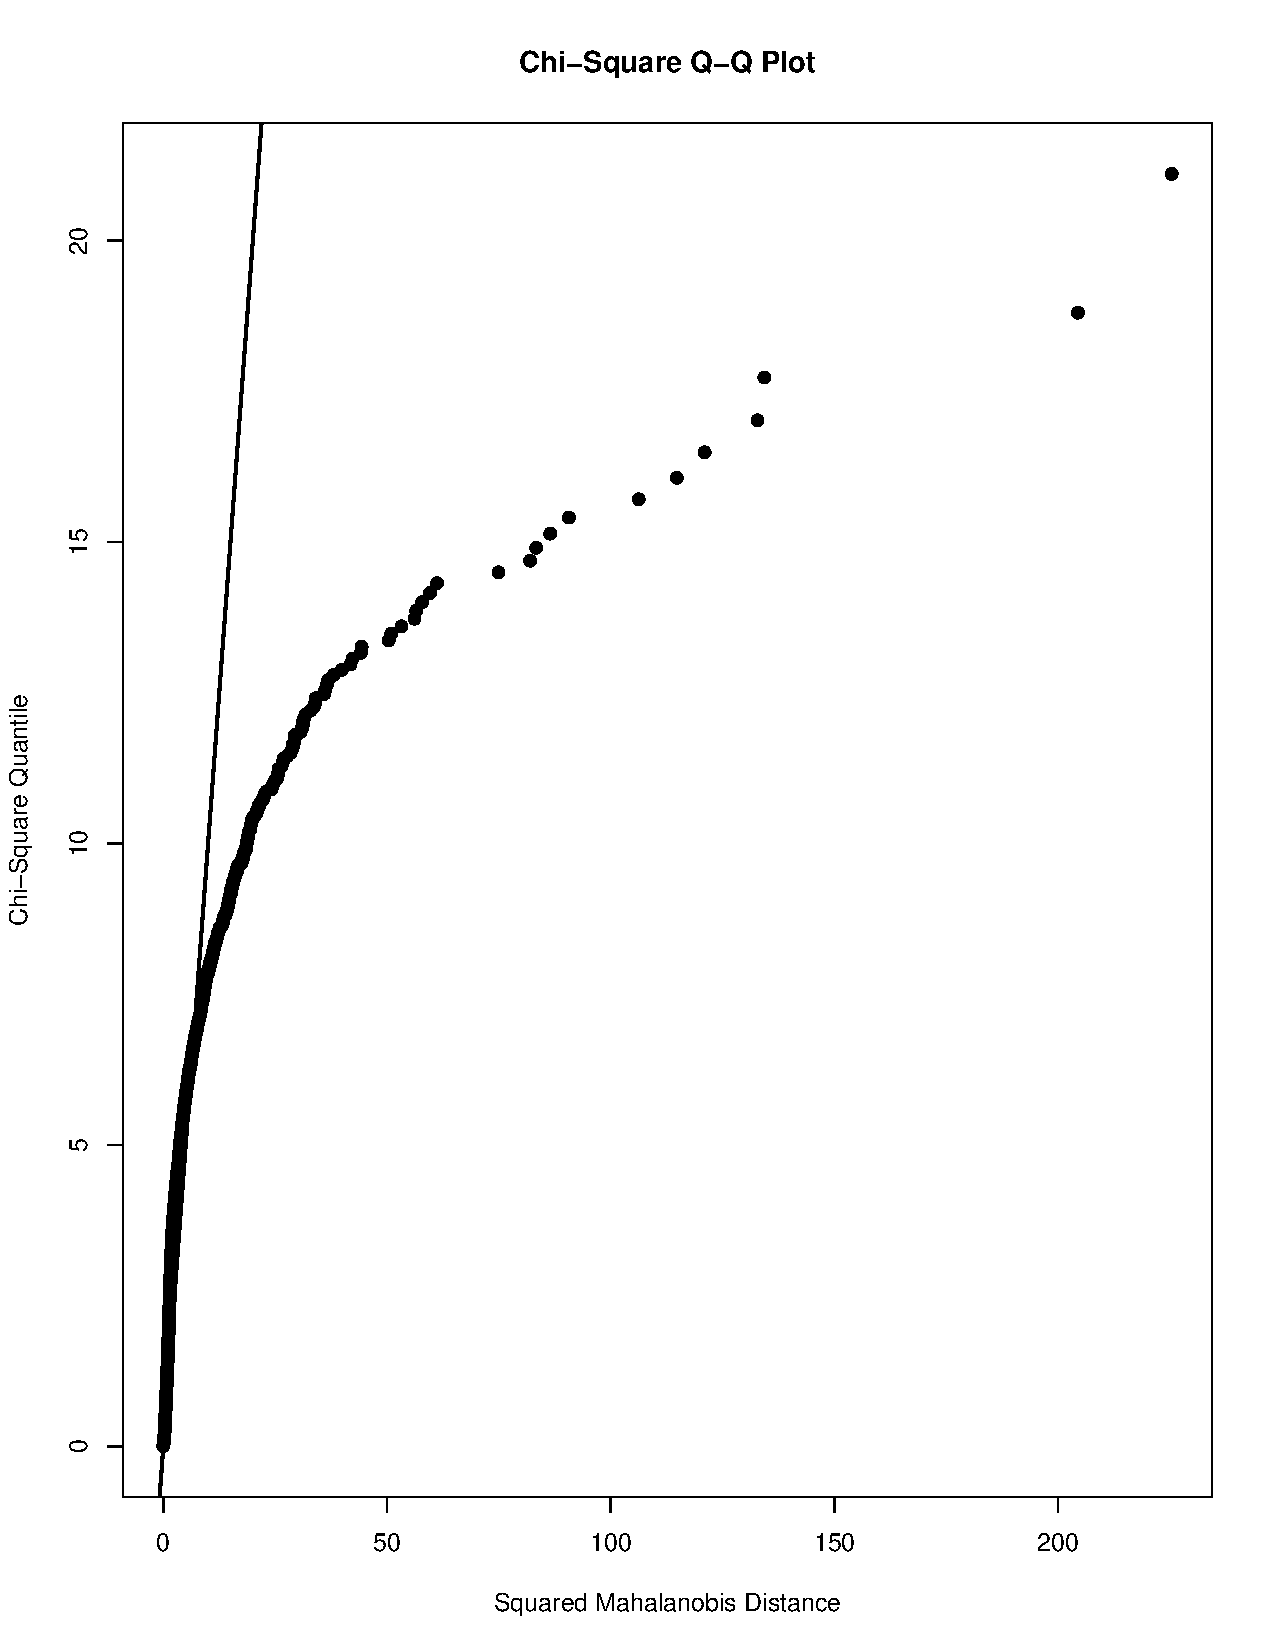
\includegraphics[width = 6.5cm,height = 6.5cm]{Figure/chisqqq.pdf}
		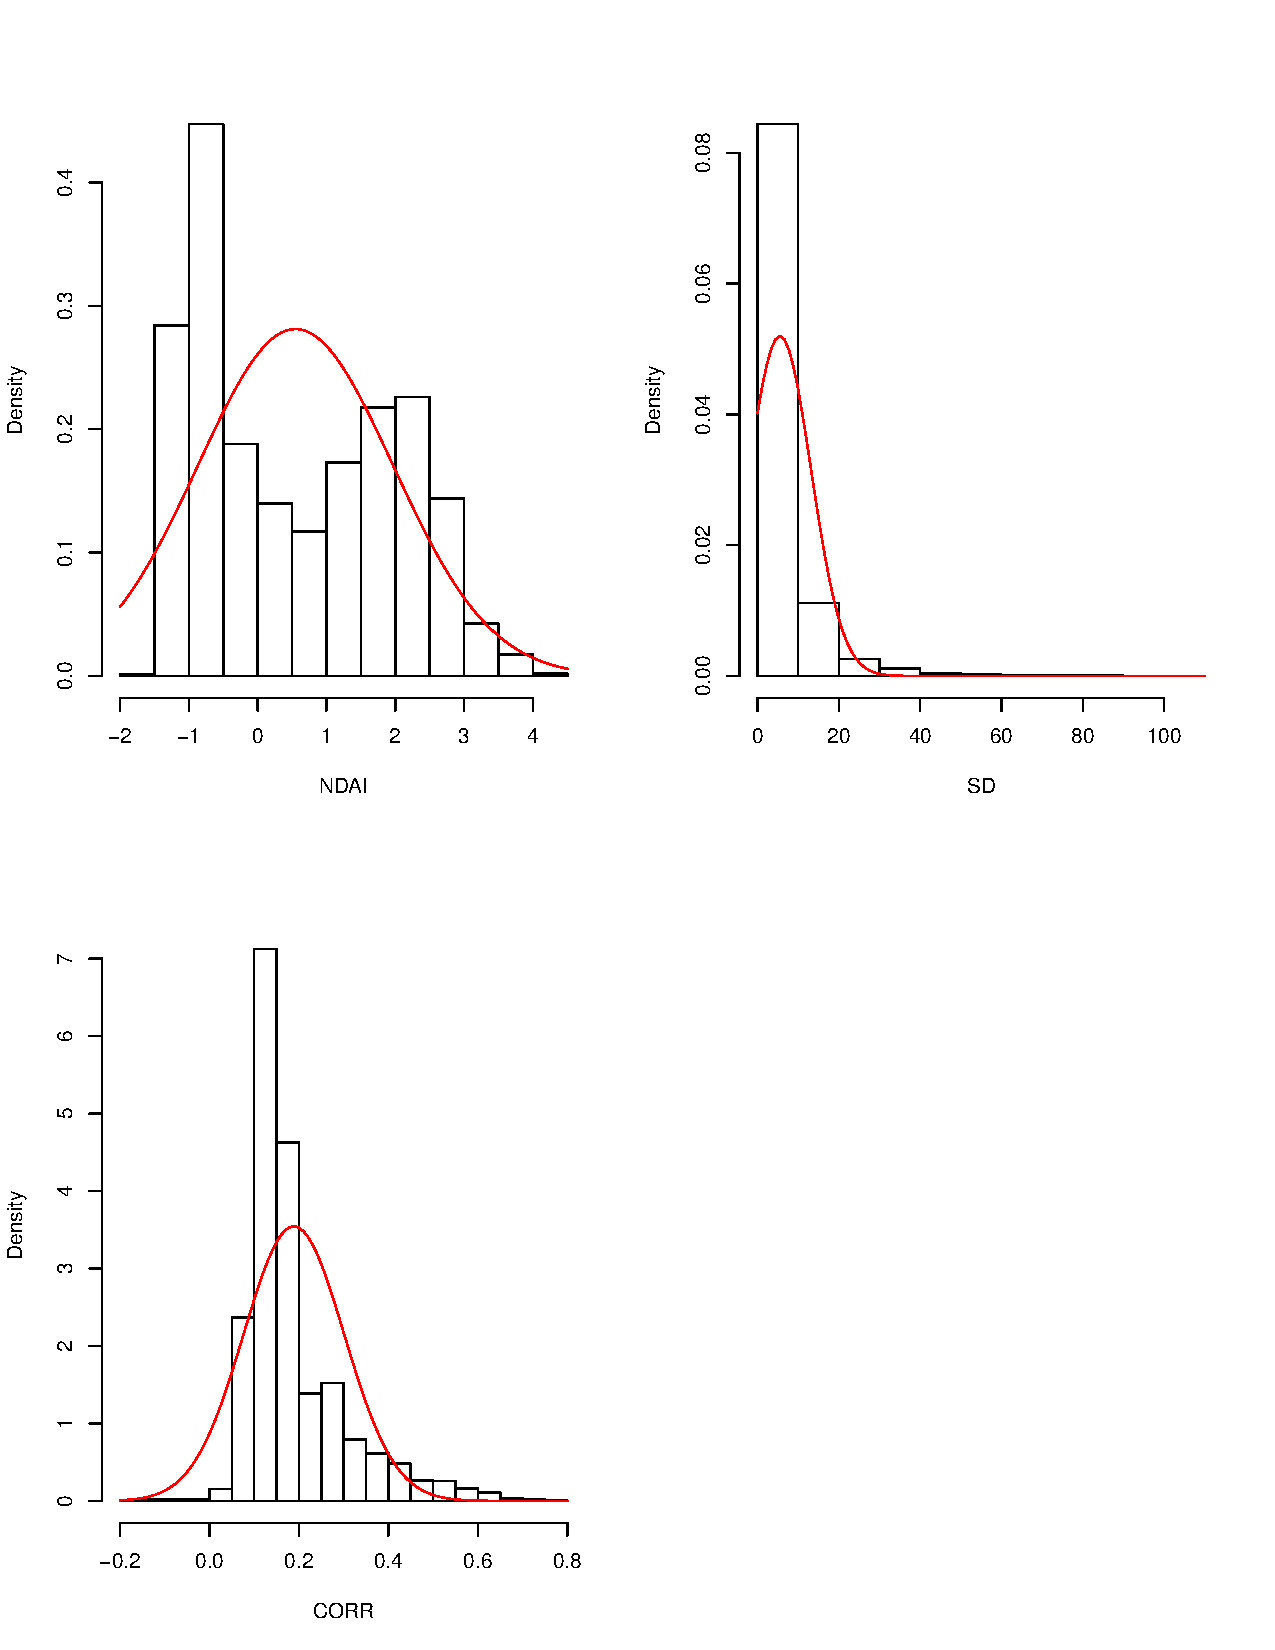
\includegraphics[width = 7cm, height = 7cm]{Figure/hist}
		\caption{Left: Chi-Square QQ plot. Right: univariate histograms.}
		\label{MVNtest}
	\end{figure}



\begin{table}[h!]
\centering
\begin{tabular}{|l|l|l|l|l|l|l|l|l|}
\cline{1-4} \cline{6-9}
     & NDAI & SD    & CORR &  &      & NDAI & SD    & CORR \\ \cline{1-4} \cline{6-9} 
NDAI & 0.44 & 2.33  & 0.02 &  & NDAI & 1.12 & 4.14  & 0.02 \\ \cline{1-4} \cline{6-9} 
SD   & 2.33 & 66.84 & 0.24 &  & SD   & 4.14 & 35.22 & 0.09 \\ \cline{1-4} \cline{6-9}
CORR & 0.02 & 0.24  & 0.02 &  & CORR & 0.02 & 0.09  & 0.01 \\ \cline{1-4} \cline{6-9} 
\end{tabular}
\caption{Covariance matrixes. Left for label 1 (cloud), right for label -1 (not cloud).}
\label{tabCovarianceMatrix}
\end{table}


	\par
	For logistic regression for two classes, we assume that $P(y=1|x) = \frac{e^{w\tp x+b}}{1+e^{w\tp x + b}}$ and $P(y=-1|x) = \frac{1}{1+e^{w\tp x + b}}$, which can be seen as approximately satisfied considering that we are doing 2-class classification. \par
	For SVM, there are no probabilistic assumptions, but we have to choose hyper-parameters here. Since training SVM is very time-consuming, we only try several values here and pick the best one based on cross validation. For Linear SVM,  we need to choose hyper-parameter $C$. We try three values $\frac{1}{3},1,3$ for it and find that $C=1$ generates the largest CV accuracy, so we choose $C=3$ for Linear SVM. For Kernel SVM with Gaussian radial function, we need to choose two hyper-parameters $C$ and $\gamma$. We try every combination of $C,\gamma\in\{\frac{1}{3},1,3\}$ and find that $C=1,\gamma=\frac{1}{3}$ generates the largest CV accuracy, so we choose $C=1,\gamma=\frac{1}{3}$ for Kernel SVM. 

	
	

\item[(ii)] Cross validation and test accuracy \par
	
	By results of cross validation in Table \ref{tabCV1},\ref{tabCV2} and test accuracy in Table \ref{tabTestAccuracy}, we can find that CV accuracy and test accuracy of all models are around $0.9$, and it is difficult to further increase the CV/test accuracy. Besides, Kernel SVM performs best with largest CV accuracy and test accuracy.
	
\begin{table}[h!] 
\centering
\begin{tabular}{|c|c|c|c|c|c|c|c|c|c|c|c|}
\hline
                                                              & \multicolumn{10}{c|}{Accuracy Across Folds}                                   & \begin{tabular}[c]{@{}c@{}}CV\\ Accuracy\end{tabular} \\ \hline
LDA                                                           & 0.876 & 0.968 & 0.898 & 0.891 & 0.897 & 0.877 & 0.894 & 0.880 & 0.896 & 0.923 & 0.901                                                 \\ \hline
QDA                                                           & 0.903 & 0.960 & 0.889 & 0.858 & 0.879 & 0.889 & 0.892 & 0.884 & 0.875 & 0.892 & 0.893                                                 \\ \hline
\begin{tabular}[c]{@{}c@{}}Logistic\\ Regression\end{tabular} & 0.865 & 0.959 & 0.875 & 0.877 & 0.897 & 0.878 & 0.891 & 0.879 & 0.899 & 0.899 & 0.892                                                 \\ \hline
Linear SVM                                                    & 0.872 & 0.968 & 0.893 & 0.894 & 0.898 & 0.875 & 0.896 & 0.880 & 0.896 & 0.925 & 0.900                                                 \\ \hline
Kernel SVM                                                    & 0.938     & 0.982     & 0.928     & 0.961     & 0.953     & 0.951     & 0.949     & 0.951     & 0.932     & 0.980     & 0.952                                                     \\ \hline
\end{tabular}
\caption{Cross validation with split method 1}
\label{tabCV1}
\end{table}

\begin{table}[h!]
\centering
\begin{tabular}{|c|c|c|c|c|c|c|c|c|c|c|c|}
\hline
                                                              & \multicolumn{10}{c|}{Accuracy Across Folds}                                   & \begin{tabular}[c]{@{}c@{}}CV\\ Accuracy\end{tabular} \\ \hline
LDA                                                           & 0.894 & 0.884 & 0.926 & 0.924 & 0.902 & 0.882 & 0.911 & 0.881 & 0.909 & 0.897 & 0.901                                                 \\ \hline
QDA                                                           & 0.880 & 0.861 & 0.912 & 0.907 & 0.901 & 0.873 & 0.908 & 0.873 & 0.923 & 0.901 & 0.894                                                 \\ \hline
\begin{tabular}[c]{@{}c@{}}Logistic\\ Regression\end{tabular} & 0.887 & 0.878 & 0.918 & 0.917 & 0.891 & 0.875 & 0.906 & 0.870 & 0.895 & 0.894 & 0.893                                                 \\ \hline
Linear SVM                                                    & 0.896 & 0.885 & 0.925 & 0.926 & 0.901 & 0.882 & 0.910 & 0.879 & 0.907 & 0.897 & 0.901                                                 \\ \hline
Kernel SVM                                                    & 0.953 & 0.955 & 0.976 & 0.968 & 0.959 & 0.943 & 0.947 & 0.931 & 0.972 & 0.955 & 0.956                                                 \\ \hline
\end{tabular}
\caption{Cross validation with split method 2}
\label{tabCV2}
\end{table}

\begin{table}[h!]
\centering
\begin{tabular}{|l|l|l|l|l|l|}
\hline
              & LDA    & QDA    & Logistic Regression & Linear SVM & Kernel SVM \\ \hline
Test Accuracy & 0.8826 & 0.8920 & 0.8739              & 0.8842     & 0.9122     \\ \hline
\end{tabular}
\caption{Test Accuracy}
\label{tabTestAccuracy}
\end{table}
	
	
\end{enumerate}



\item ROC curves \par
	By ROC curves in Figure \ref{ROC} we can find that all models perform well since all of them have AUC around 0.95, while Kernel SVM appears to perform best with a largest AUC=0.9608. \\
	Here, we choose the cutoff value to be 0.5. For one thing, it is reasonable and natural to classify one observation to be cloud when the probability of being cloud is larger or equal to 0.5. For another, from plots we can see that by choosing the cutoff value 0.5 we can maintain a relatively high True Positive Fraction while keeping False Positive Fraction relatively low.
	
\begin{figure}[h!]
	\centering
	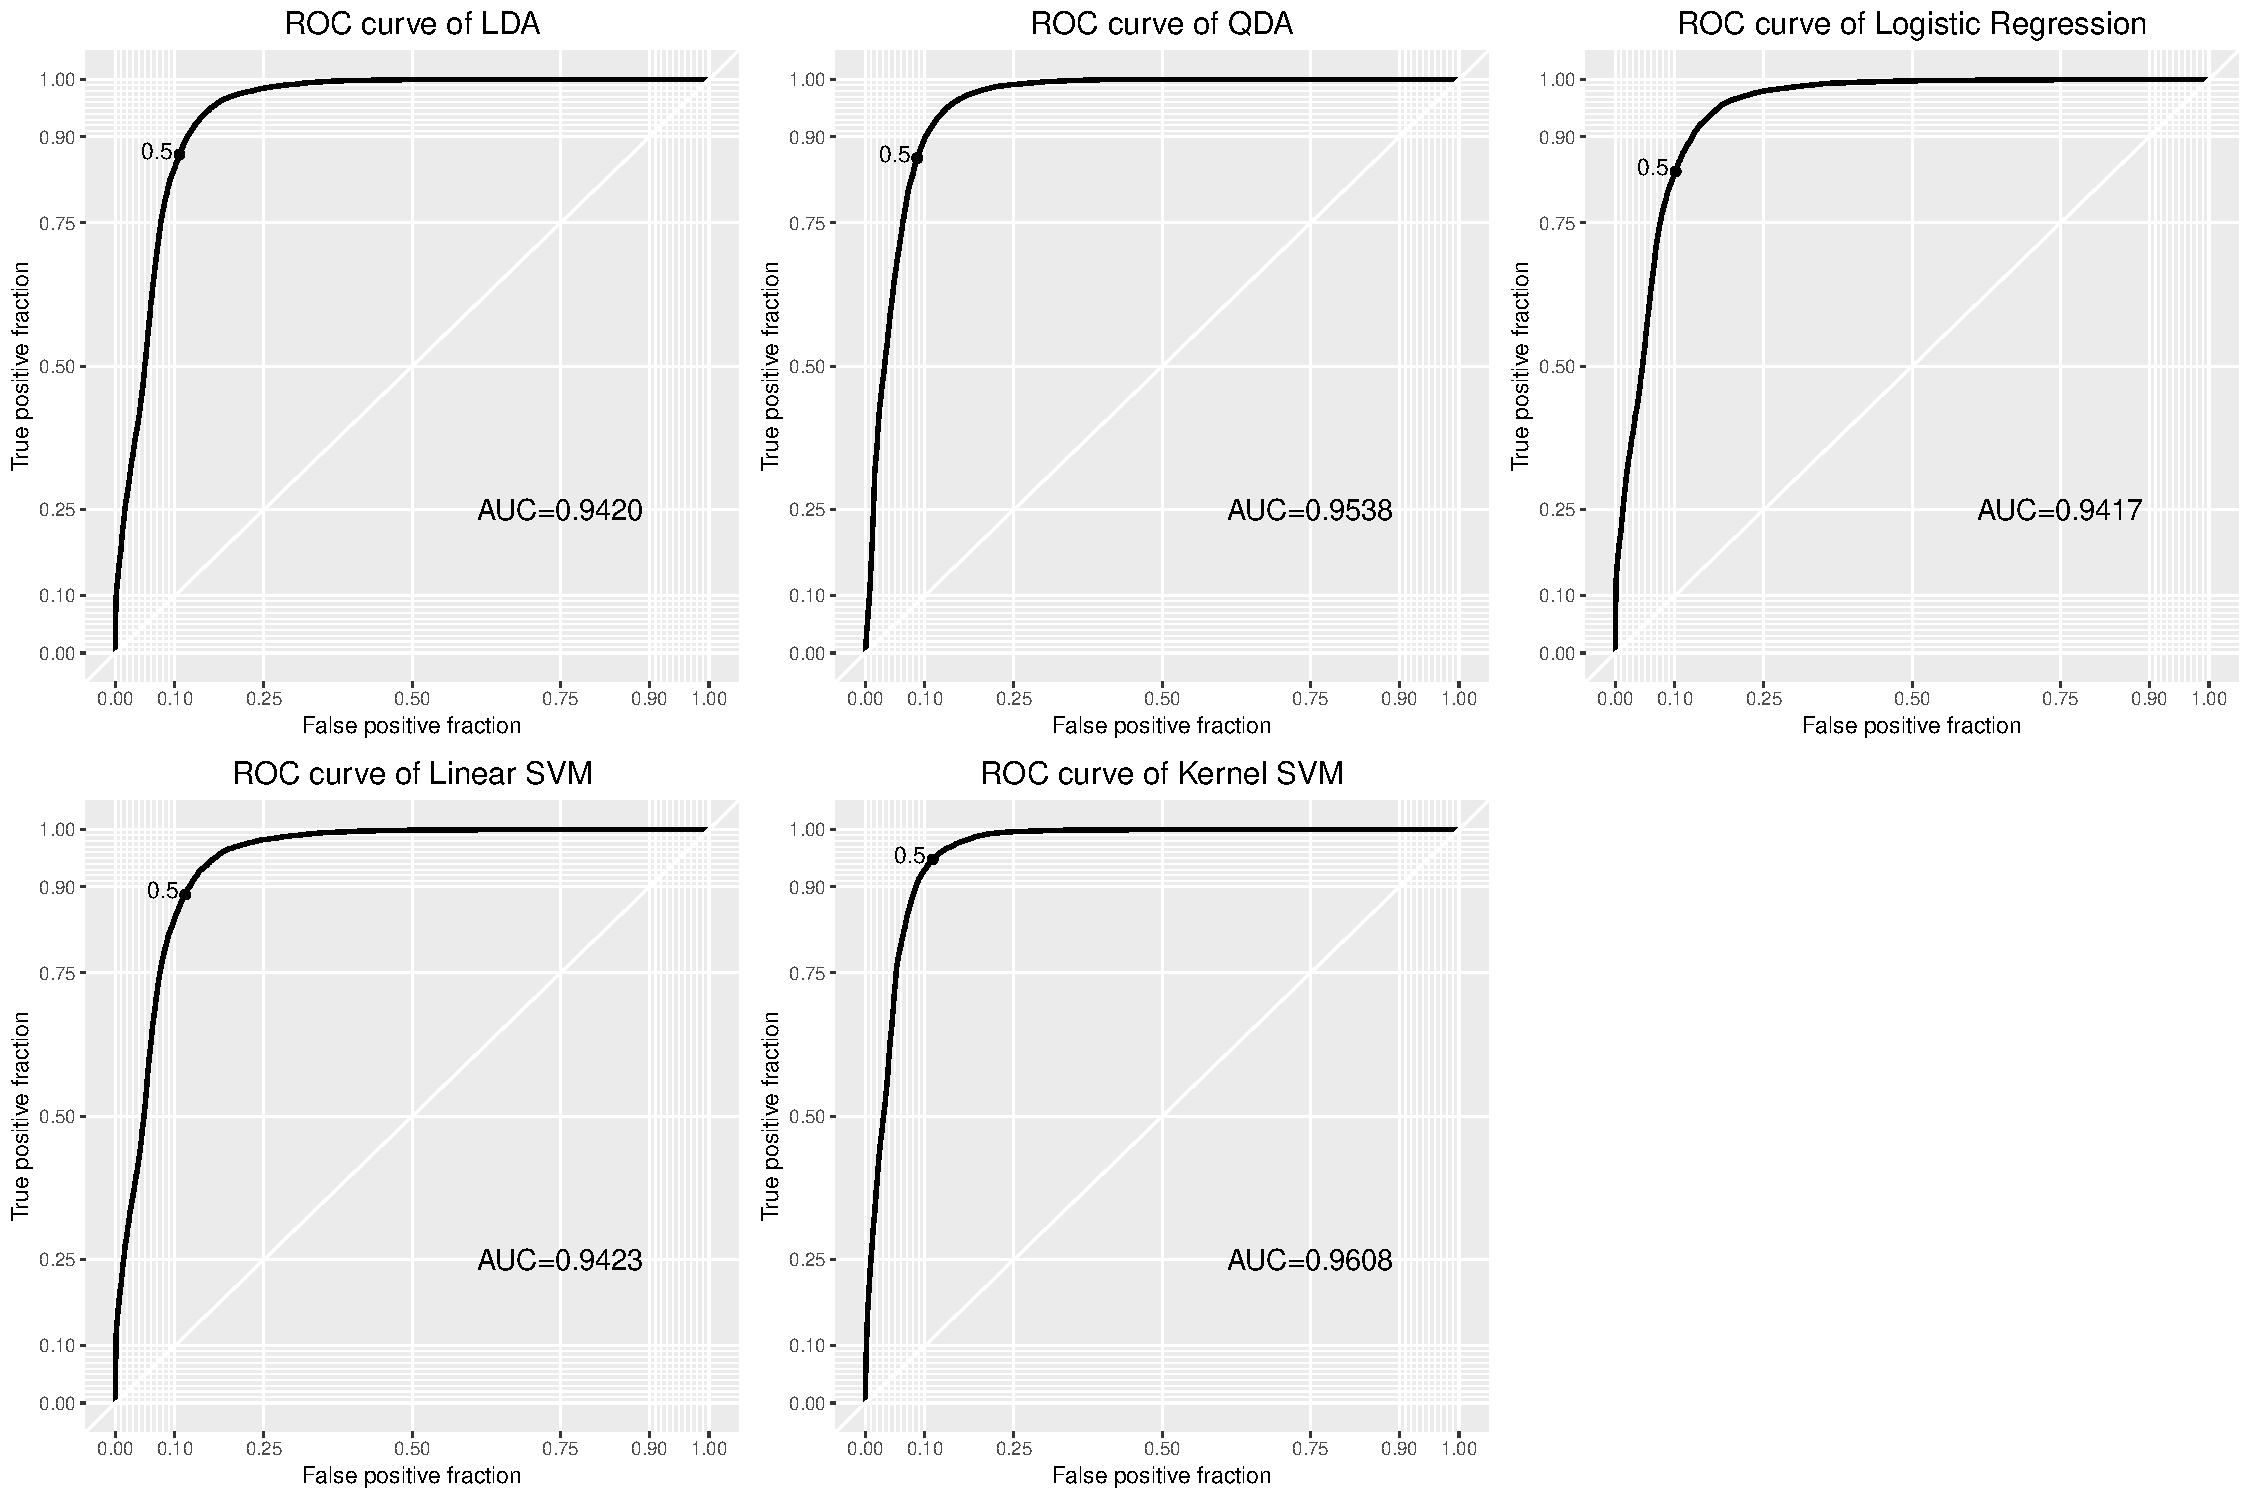
\includegraphics[height = 8cm]{Figure/ROC.pdf}
	\caption{ROC curves}
	\label{ROC}
\end{figure}

\item Assess models by Confusion Matrix and F1 score \par

	By confusion matrixes of all methods in Table \ref{tabConfusionMatrix} we can find that Kernel SVM has a significant small False Negative value compared with other methods. \\
	F1 score, defined by the harmonic average of the precision and recall, is a measure of accuracy. With results in Table \ref{tabF1} We find that Kernel SVM has the largest F1 score.

\begin{table}[h!]
\centering
\begin{tabular}{lllllllll}
\cline{1-4} \cline{6-9}
\multicolumn{2}{|l|}{\multirow{2}{*}{LDA}}                                                                                                                                   & \multicolumn{2}{l|}{Actual Label}                                                                     & \multicolumn{1}{l|}{} & \multicolumn{2}{l|}{\multirow{2}{*}{QDA}}                                                                                                                                  & \multicolumn{2}{l|}{Actual Label}                                                                     \\ \cline{3-4} \cline{8-9} 
\multicolumn{2}{|l|}{}                                                                                                                                                       & \multicolumn{1}{l|}{Cloud} & \multicolumn{1}{l|}{\begin{tabular}[c]{@{}l@{}}Not\\ Cloud\end{tabular}} & \multicolumn{1}{l|}{} & \multicolumn{2}{l|}{}                                                                                                                                                      & \multicolumn{1}{l|}{Cloud} & \multicolumn{1}{l|}{\begin{tabular}[c]{@{}l@{}}Not\\ Cloud\end{tabular}} \\ \cline{1-4} \cline{6-9} 
\multicolumn{1}{|l|}{\multirow{2}{*}{\begin{tabular}[c]{@{}l@{}}Predicted \\ Label\end{tabular}}} & \multicolumn{1}{l|}{Cloud}                                               & \multicolumn{1}{l|}{16089} & \multicolumn{1}{l|}{2777}                                                & \multicolumn{1}{l|}{} & \multicolumn{1}{l|}{\multirow{2}{*}{\begin{tabular}[c]{@{}l@{}}Predicted\\ Label\end{tabular}}} & \multicolumn{1}{l|}{Cloud}                                               & \multicolumn{1}{l|}{15969} & \multicolumn{1}{l|}{2240}                                                \\ \cline{2-4} \cline{7-9} 
\multicolumn{1}{|l|}{}                                                                            & \multicolumn{1}{l|}{\begin{tabular}[c]{@{}l@{}}Not\\ Cloud\end{tabular}} & \multicolumn{1}{l|}{2412}  & \multicolumn{1}{l|}{22914}                                               & \multicolumn{1}{l|}{} & \multicolumn{1}{l|}{}                                                                           & \multicolumn{1}{l|}{\begin{tabular}[c]{@{}l@{}}Not\\ Cloud\end{tabular}} & \multicolumn{1}{l|}{2532}  & \multicolumn{1}{l|}{23451}                                               \\ \cline{1-4} \cline{6-9} 
                                                                                                  &                                                                          &                            &                                                                          &                       &                                                                                                 &                                                                          &                            &                                                                          \\ \cline{1-4} \cline{6-9} 
\multicolumn{2}{|l|}{\multirow{2}{*}{Logistic Regression}}                                                                                                                   & \multicolumn{2}{l|}{Actual Label}                                                                     & \multicolumn{1}{l|}{} & \multicolumn{2}{l|}{\multirow{2}{*}{Linear SVM}}                                                                                                                           & \multicolumn{2}{l|}{Actual Label}                                                                     \\ \cline{3-4} \cline{8-9} 
\multicolumn{2}{|l|}{}                                                                                                                                                       & \multicolumn{1}{l|}{Cloud} & \multicolumn{1}{l|}{\begin{tabular}[c]{@{}l@{}}Not\\ Cloud\end{tabular}} & \multicolumn{1}{l|}{} & \multicolumn{2}{l|}{}                                                                                                                                                      & \multicolumn{1}{l|}{Cloud} & \multicolumn{1}{l|}{\begin{tabular}[c]{@{}l@{}}Not\\ Cloud\end{tabular}} \\ \cline{1-4} \cline{6-9} 
\multicolumn{1}{|l|}{\multirow{2}{*}{\begin{tabular}[c]{@{}l@{}}Predicted\\ Label\end{tabular}}}  & \multicolumn{1}{l|}{Cloud}                                               & \multicolumn{1}{l|}{15537} & \multicolumn{1}{l|}{2608}                                                & \multicolumn{1}{l|}{} & \multicolumn{1}{l|}{\multirow{2}{*}{\begin{tabular}[c]{@{}l@{}}Predicted\\ Label\end{tabular}}} & \multicolumn{1}{l|}{Cloud}                                               & \multicolumn{1}{l|}{16402} & \multicolumn{1}{l|}{3017}                                                \\ \cline{2-4} \cline{7-9} 
\multicolumn{1}{|l|}{}                                                                            & \multicolumn{1}{l|}{\begin{tabular}[c]{@{}l@{}}Not\\ Cloud\end{tabular}} & \multicolumn{1}{l|}{2964}  & \multicolumn{1}{l|}{23083}                                               & \multicolumn{1}{l|}{} & \multicolumn{1}{l|}{}                                                                           & \multicolumn{1}{l|}{\begin{tabular}[c]{@{}l@{}}Not\\ Cloud\end{tabular}} & \multicolumn{1}{l|}{2099}  & \multicolumn{1}{l|}{22674}                                               \\ \cline{1-4} \cline{6-9} 
                                                                                                  &                                                                          &                            &                                                                          &                       &                                                                                                 &                                                                          &                            &                                                                          \\ \cline{1-4}
\multicolumn{2}{|c|}{\multirow{2}{*}{Kernel SVM}}                                                                                                                            & \multicolumn{2}{l|}{\begin{tabular}[c]{@{}l@{}}Actual\\ Label\end{tabular}}                           &                       &                                                                                                 &                                                                          &                            &                                                                          \\ \cline{3-4}
\multicolumn{2}{|c|}{}                                                                                                                                                       & \multicolumn{1}{l|}{Cloud} & \multicolumn{1}{l|}{\begin{tabular}[c]{@{}l@{}}Not\\ Cloud\end{tabular}} &                       &                                                                                                 &                                                                          &                            &                                                                          \\ \cline{1-4}
\multicolumn{1}{|l|}{\multirow{2}{*}{\begin{tabular}[c]{@{}l@{}}Predicted\\ Label\end{tabular}}}  & \multicolumn{1}{l|}{Cloud}                                               & \multicolumn{1}{l|}{17534} & \multicolumn{1}{l|}{2912}                                                &                       &                                                                                                 &                                                                          &                            &                                                                          \\ \cline{2-4}
\multicolumn{1}{|l|}{}                                                                            & \multicolumn{1}{l|}{\begin{tabular}[c]{@{}l@{}}Not\\ Cloud\end{tabular}} & \multicolumn{1}{l|}{967}   & \multicolumn{1}{l|}{22779}                                               &                       &                                                                                                 &                                                                          &                            &                                                                          \\ \cline{1-4}
\end{tabular}
\caption{Confusion Matrixes}
\label{tabConfusionMatrix}
\end{table}

\begin{table}[!htb]
\centering
\begin{tabular}{|l|l|l|l|l|l|}
\hline
         & LDA    & QDA    & Logistic Regression & Linear SVM & Kernel SVM \\ \hline
F1 Score & 0.8611 & 0.8700 & 0.8480              & 0.8651     & 0.9004     \\ \hline
\end{tabular}
\caption{F1 scores}
\label{tabF1}
\end{table}

	
\end{enumerate}

\section{Diagnostics}
In previous part, we find that Kernel SVM with Gaussian radial function appears to perform best among all the models, so we do diagnostics for Kernel SVM in this part.
\begin{enumerate}[label=(\alph*)]
\item Diagnostic plot \\
	\begin{figure}[h!]
		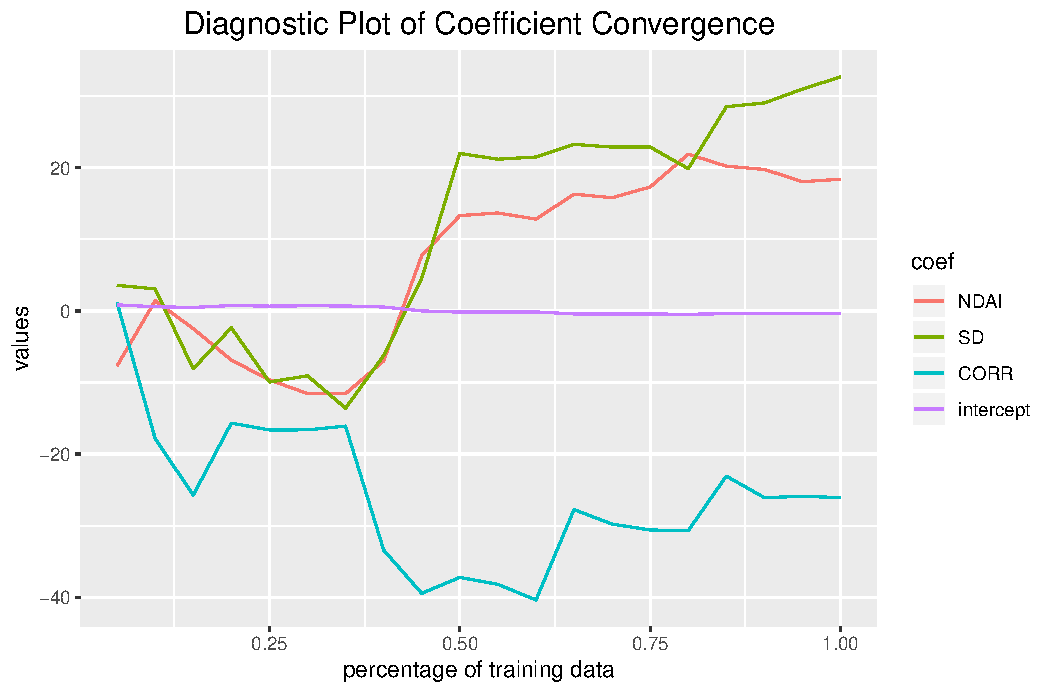
\includegraphics[width = 8cm,height = 5cm]{Figure/diag1}
		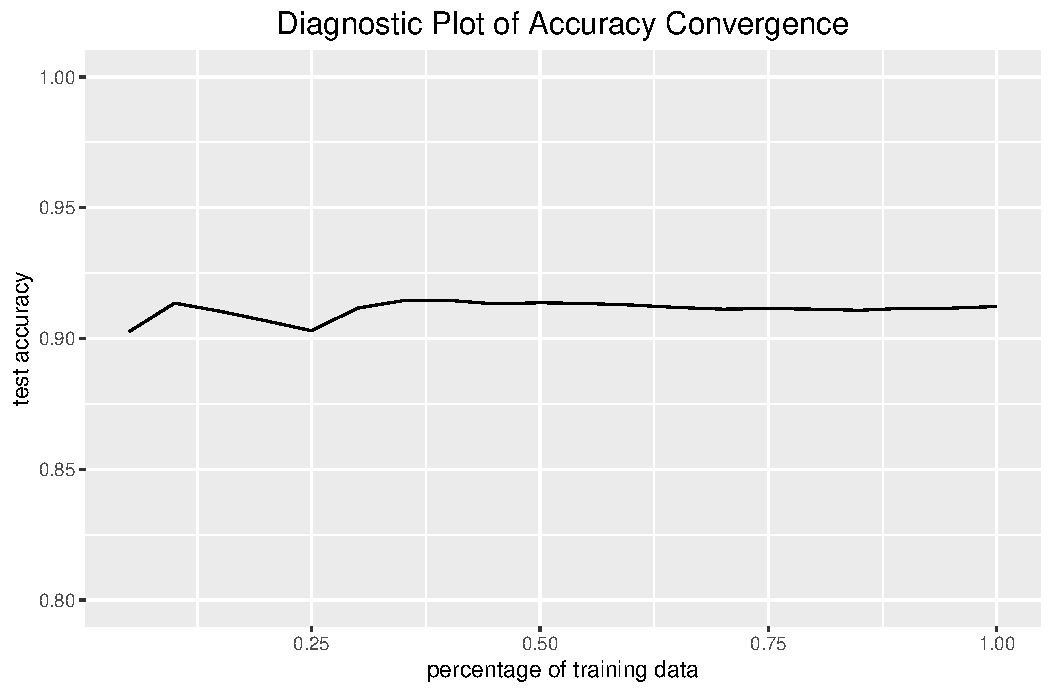
\includegraphics[width = 7cm,height = 5cm]{Figure/diag2}
		\caption{Left: Plot of coefficient convergence. Right: Plot of accuracy convergence.}
		\label{diag}
	\end{figure}
	From the plot of coefficient convergence in Figure \ref{diag}, though we can not determine whether the coefficients are going to converge, we can find that they appear to be less volatile (less variance) as we increase traing data. \\
	From the plot of accuracy convergence in Figure \ref{diag}, we can find that the test accuracy gradually converge to around 0.91.
	
\item Analysis of misclassified data \\
	\begin{figure}[h!]
		\centering
		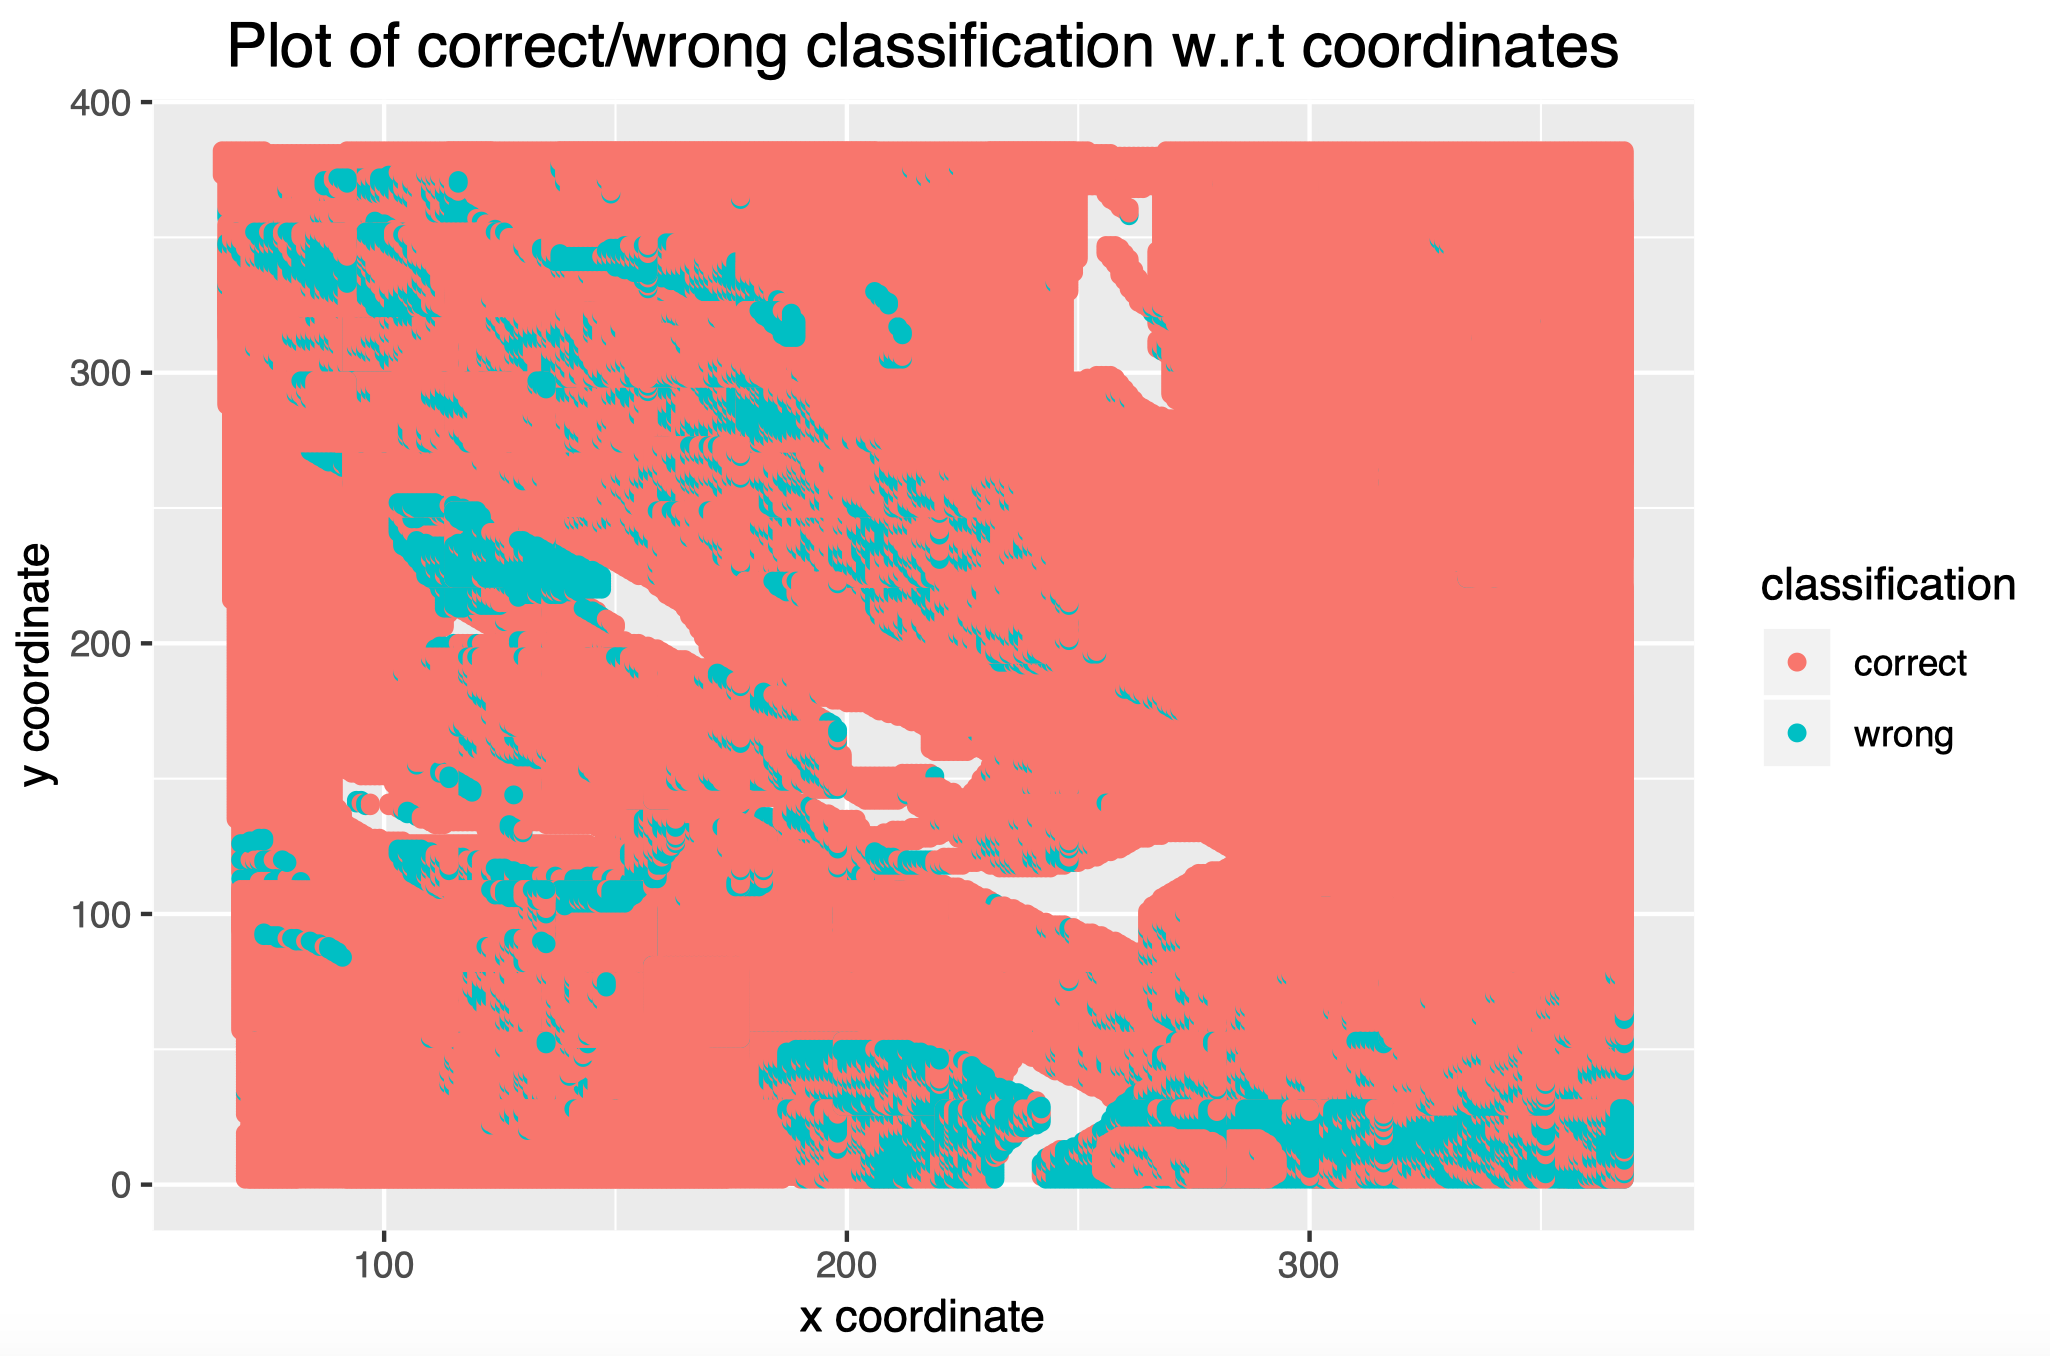
\includegraphics[width = 10cm]{Figure/coor}
		\caption{Plot of correct/Wrong classified data with coordinates}
		\label{coor}
	\end{figure}
	First, we plot correct and wrong classified data with respect to x and y coordinates in Figure \ref{coor} (including both training and test set). Some blank area occur since we exclude unlabeled data before training and testing models, so they do not show up. The misclassified data are mainly in lower triangular part of the plot, but we do not find a specific pattern here.\\
	\begin{figure}[h!]
		\centering
		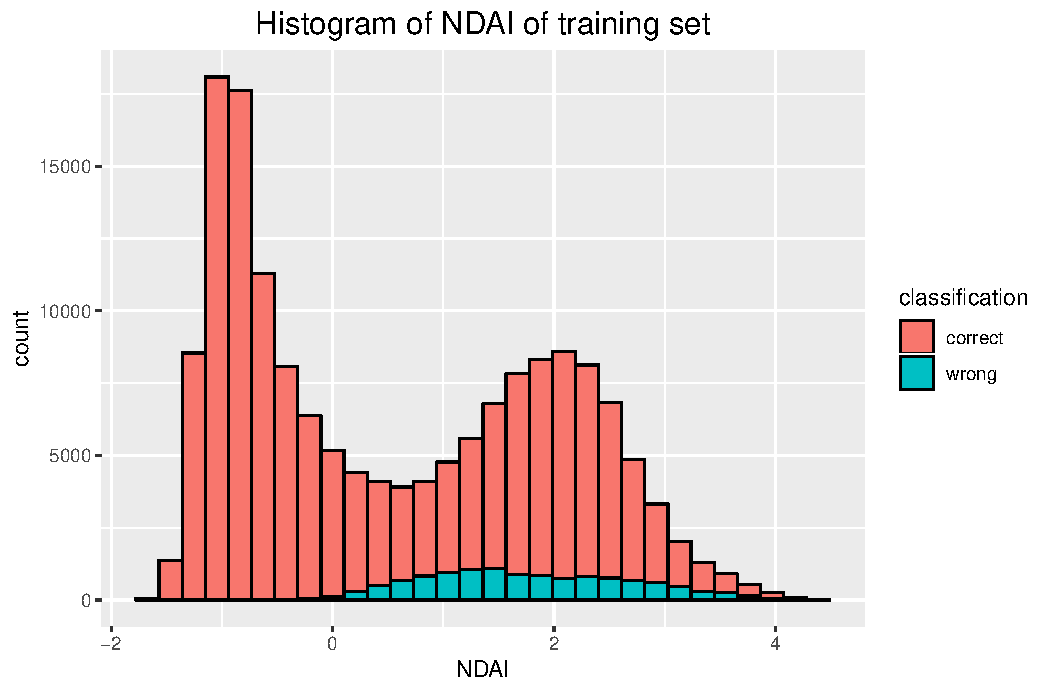
\includegraphics[width = 7.5cm]{Figure/hist1}
		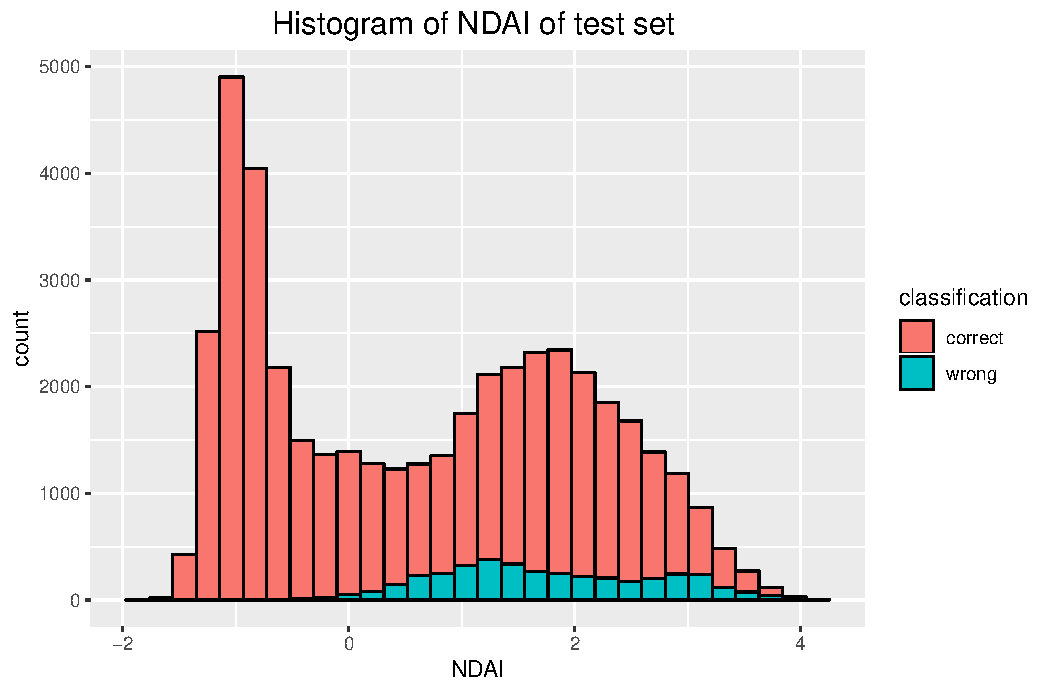
\includegraphics[width = 7.5cm]{Figure/hist2}
		\caption{Left: Histogram of NDAI of training set. Right: Histogram of NDAI of test set.}
		\label{hist}
	\end{figure}
	Then we plot the histograms of every feature, and find it interesting for NDAI in Figure \ref{hist}. Here we plot histograms of NDAI with respect to right/wrong classified data for training set and test set separately. We can find that the misclassified data have NDAI mainly between 0 and 4, and for data with NDAI less than 0, we almost correctly classify all of them.
\item A better classifier, mixture of models \\
	In previous part, we can see that a specific model has its limitation. So we design a mixture of models and see how it performs. Basically, we let each model vote for classification based on its results and each model has a weight for its vote. Based on their performance in part 3, we choose a mixture of QDA and kernel SVM and set the weight to be $0.5,0.5$ respectively, which sum up to one. We classify an observation to be cloud (+1) if it gets score larger or equal to $0.5$. And note that we should not assign a weight larger than $0.5$ for one model, otherwise that model will dominate and the mixture will be no different from a single model. We also do cross validation in Table \ref{tabCVmixture} and find test accuracy is $0.9128$ for our mixture model. We can find that the test accuracy of mixture model is better than any single model, but for CV accuracy, mixture model is not as good as but close to Kernel SVM and still better than any other single model. Therefore, we expect our mixture model to work at least as good as, probably better than, any single model we have tried in part 3.

\begin{table}[h!]
\centering
\begin{tabular}{|c|c|c|c|c|c|c|c|c|c|c|c|}
\hline
                                                        & \multicolumn{10}{c|}{Accuracy Across Folds}                                   & \begin{tabular}[c]{@{}c@{}}CV\\ Accuracy\end{tabular} \\ \hline
\begin{tabular}[c]{@{}c@{}}Mixture\\ Model\end{tabular} & 0.921 & 0.983 & 0.932 & 0.945 & 0.913 & 0.909 & 0.911 & 0.883 & 0.913 & 0.990 & 0.930                                                 \\ \hline
\end{tabular}
\caption{Cross validation of mixture model}
\label{tabCVmixture}
\end{table}


\item The results remain almost same as we change the way of splitting data as shown in figure \ref{changesplit}.

\begin{figure}[h!]
	\centering
	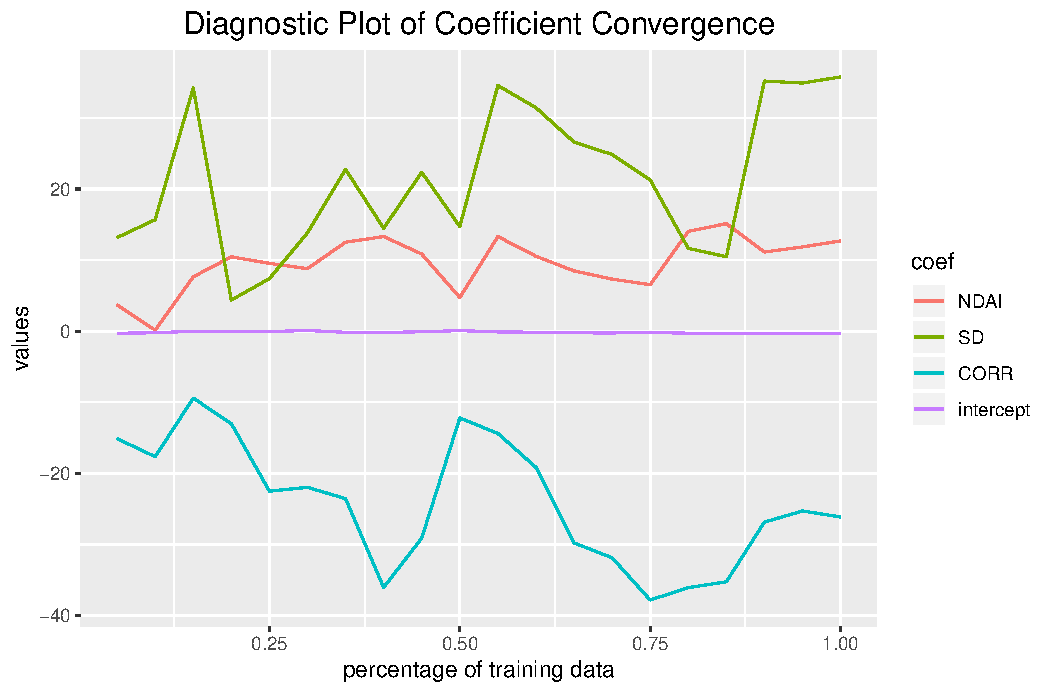
\includegraphics[width = 5cm,height = 3cm]{Figure/m1}
	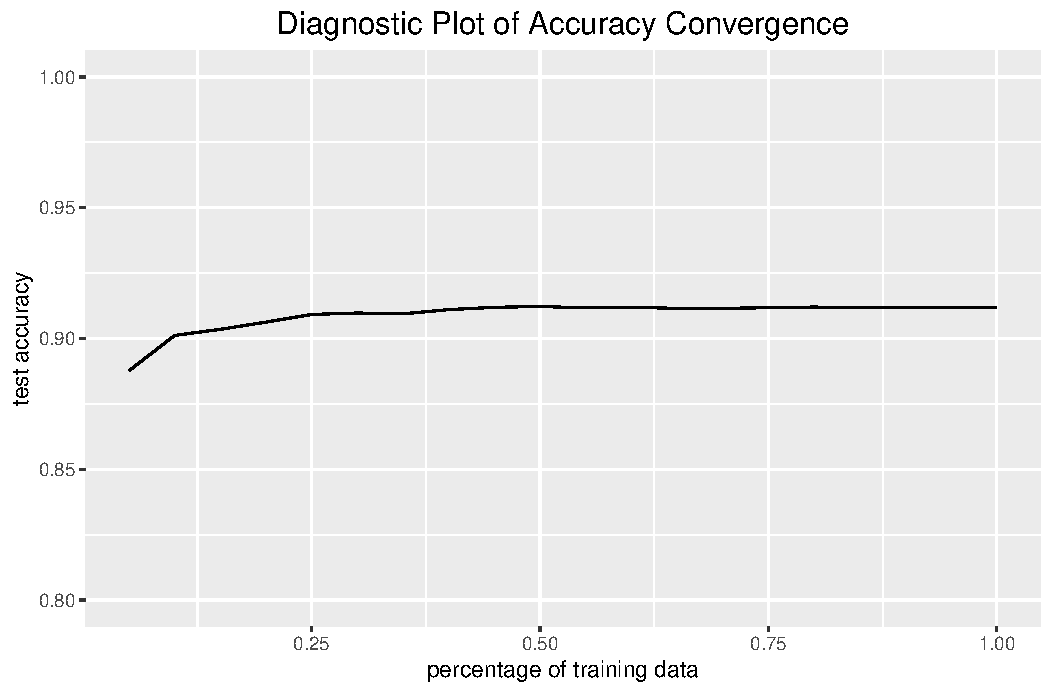
\includegraphics[width = 4cm,height = 3cm]{Figure/m2} 
	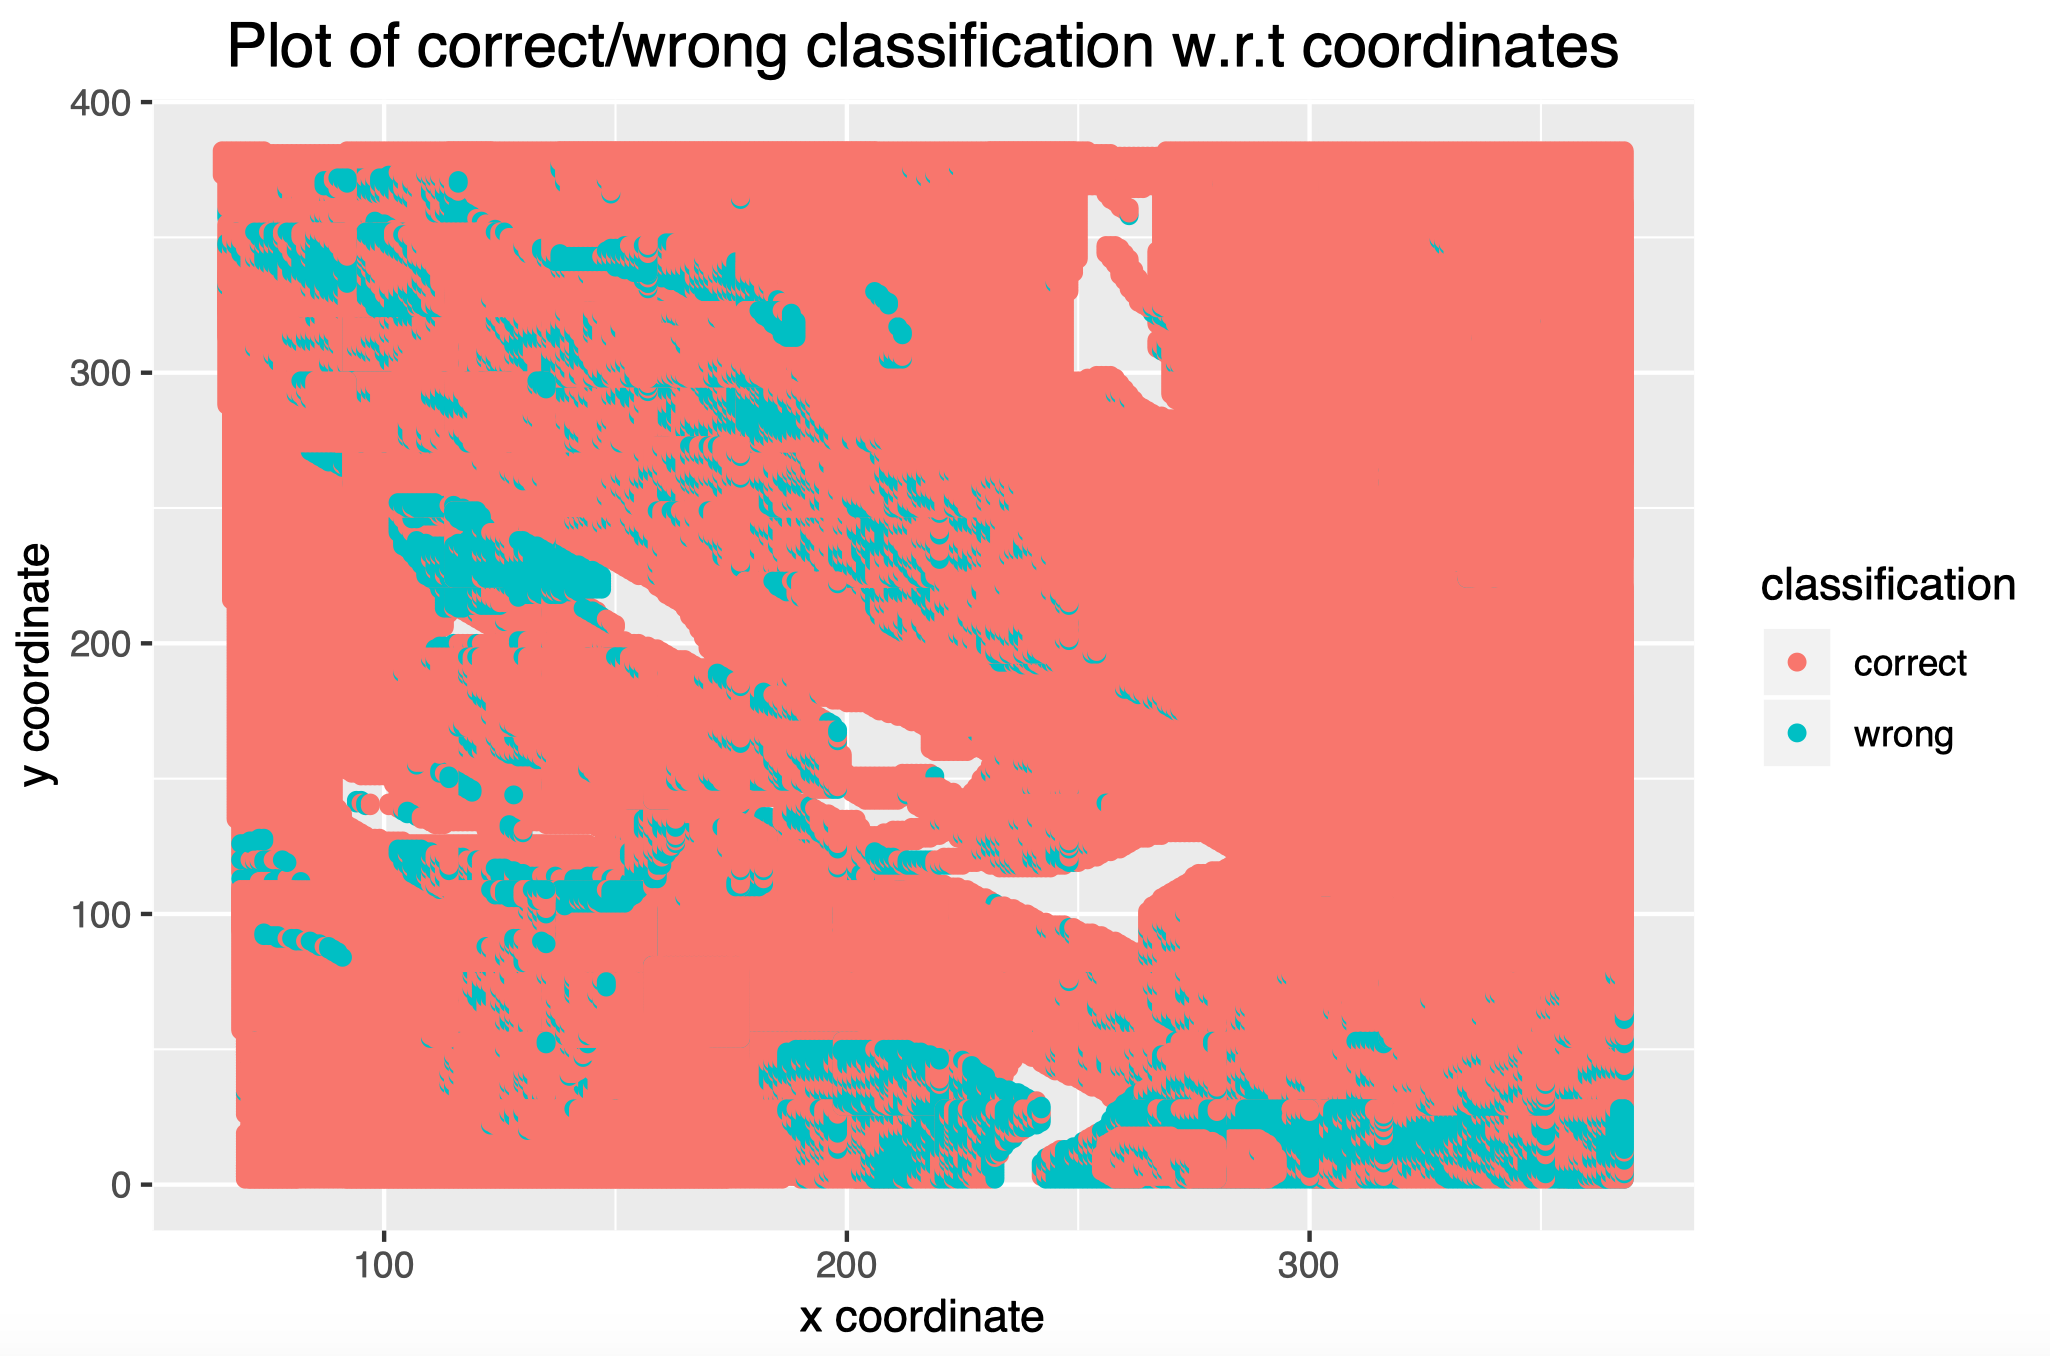
\includegraphics[width = 4cm, height = 3cm]{Figure/coor}
	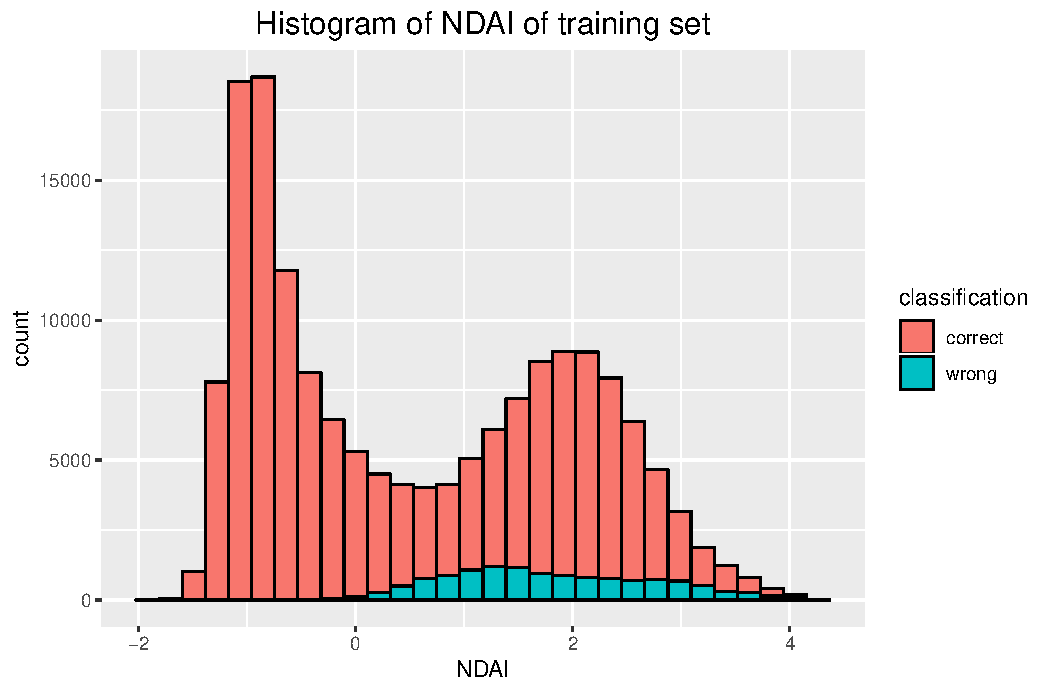
\includegraphics[width = 5cm]{Figure/hist1prime}
	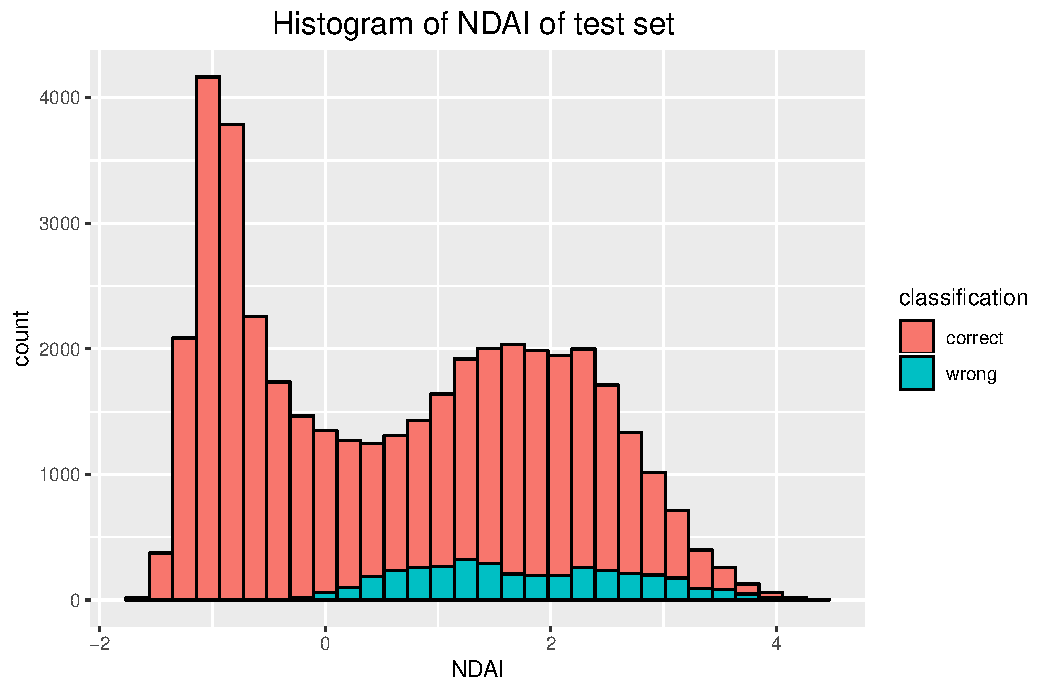
\includegraphics[width = 5cm]{Figure/hist2prime}
	\caption{Plots when changing the way of splitting data}
	\label{changesplit}
\end{figure}


\item Conclusion \\
	In this part, we first do diagnostic analysis on our best model Kernel SVM and find that parameters seem to get stable and less volatile and test accuracy appears to converge as we increase training data. Then we find some certain patterns for our misclassified data. In (c), we come up with a new model, a mixture of all our models in part 3, and find it performs better.
\end{enumerate}

\section{Reproducibility}
\qquad \; All project relevant materials on github:\par
\quad \href{https://github.com/HuaBron/Ucb_Stat154_Project2}{\textbf{https://github.com/HuaBron/Ucb\_Stat154\_Project2}}

\newpage

\section*{Acknowledge section}
\quad In the process of completing this project, we discuss, interchange our thoughts and to be more efficient, we divided to focus on different parts. The specific allocation about five sections is listed as following:
\begin{enumerate}
	\item[] Section 1: Zhihua Zhang
	\item[] Section 2: Zhihua Zhang
	\item[] Section 3: Yang Xiang
	\item[] Section 4: Yang Xiang
	\item[] Section 5: Zhihua Zhang
\end{enumerate}
\quad During finishing this project, we refer to different resources like R document "trainModelList" \cite{RtrainModelList}, Wikipedia article about SVM \cite{SVMwiki} and a simple realization about logistic regression \cite{LogisticExample} for help.\par
\quad To proceed our project, we first read the reference paper carefully, exchange views and try to reach accordance. Because the data is cleaned, we then begin to do visualization and EDA. By simply plotting the well-labeled map according to expert labels(including the uncertain data), we observe the existence of spatial dependency, which indicates data is non i.i.d here. In view of this, instead of splitting data randomly, we do block-sampling to divide. To be specific, it includes partitioning data into blocks to remain dependency and then doing random sampling. The size of block is the key parameter to consider. After that, we check the performance of trivial classifier and find out this problem is non trivial. As good features are crucial to obtain higher accuracy, we then select them through quantitative and visual justification. Finally we decide to use best three $NDAI$, $SD$ and $CORR$. Moreover, we design our customized generic CV function which can fit many models like lda, qda, logistic regression and svm, and reports final and individual fold accuracy.\par
\quad We compare the performance of different methods, including LDA, QDA, Logistic Regression, Linear SVM and Kernel SVM, through cross validation, ROC curve, confusion matrix and F1 score, and find that Kernel SVM appears to perform best. Then, in part 4, we do diagnostic analysis on Kernel SVM, including convergence of parameters and patterns of misclassified data. We try to come up with a better model by using combination of our models to form a mixture model and find it performs well.







\renewcommand\refname{} 
\bibliographystyle{unsrt} 
\bibliography{library.bib}


\end{document}
